
\chapter{概形的有用态射类}
\label{ch:useful-morphisms}

我们现在要定义多得过剩的种种态射类型。有些性质（常为有限性性质）之所以有用，是因为多数「合理」的态射都带有它们，它们将在证明中以显然的方式被使用。另一些则对应几何上有意义的行为，你应当对每一种的含义都有一幅图景。

\textbf{8.0.1.\ 视角转换：态射比对象更基本。}\quad \trGrothendieck{}的一课是：我们常常当作对象之性质的东西，更好地被理解为态射的性质。把对象性质转化为态射性质的一种办法如下：若 $P$ 是\trScheme{}的一条性质，我们便（往往——但并非总\textsuperscript{1}——如此）说\trMorphism{} $\pi\colon X\to Y$ 具有 $P$，如果对 $Y$ 的每个\trAffine\trOpenSubset{} $U\subset Y$，$\pi^{-1}(U)$ 都具有 $P$。对 $P$＝\trQuasicompact、\trQuasiSeparated、\trAffine{}等，我们都将见到这种情形。（如你所望，在好的情形下，$P$ 将满足仿射通信引理~5.3.2 的两条假设，从而无须逐一检验每个仿射开子集。）不严格地说，你可以把这样的\trMorphism{}想成「所有\trFiber{}都具有 $P$」的那一种。（你现在就能把\trMorphism{}的\trFiber{}定义为拓扑空间，但等定义了\trFiberProduct{}之后，我们还会定义概形论的\trFiber{}，那时这段讨论才算真正落位。）但它的含义还不止于此：「具有 $P$」并不真是逐\trFiber{}的事，而是随\trFiber{}变化也表现良好。（作为对照：「\trManifold{}的\trSubmersion{}」的含义也多于诸\trFiber{}皆\trSmooth{}。）


\section{「合理」的态射类（如开嵌入）}

\textbf{8.1.1.}\ 你会注意到，几乎所有有用的态射类都享有许多共同的性质，而这些性质都可以由下面三条基本性质推出。我们把满足这些性质的任何一个态射类，称为概形之间态射的一个\textbf{「合理」类}（"reasonable" class of morphisms）。（为免任何愚蠢的情形，我们假定该类包含全部同构；不过这条要求还不配拥有一个属于自己的号码。）
\begin{enumerate}[label=(\roman*)]
  \item 该类\textbf{对\trComposition{}保持}：若 $\pi\colon X\to Y$ 与 $\rho\colon Y\to Z$ 都属于此类，则 $\rho\circ\pi$ 亦然。
  \item 该类\textbf{对「\trBaseChange」保持}（或「\trPullback」或「\trFiberProduct」）。确切地说：若 $\pi\colon X\to Y$ 属于此类，则对任意的 $Y'\to Y$，所诱导的映射 $X\times_Y Y'\to Y'$ 也属于此类。（这句话隐含了\trFiberProduct{} $X\times_Y Y'$ 存在的意思；但我们很快就会看到，概形的一切\trFiberProduct{}都存在，\S10.1。）
  \item 该类是\textbf{对目标局部的}（local on the target）。换言之：(a) 若 $\pi\colon X\to Y$ 属于此类，则对 $Y$ 的任意\trOpenSubset{} $V$，限制后的态射 $\pi^{-1}(V)\to V$ 属于此类；(b) 对态射 $\pi\colon X\to Y$，若存在 $Y$ 的一个\trOpenCover{} $\{V_i\}$，使得每个限制后的态射 $\pi^{-1}(V_i)\to V_i$ 都属于此类，则 $\pi$ 属于此类。特别地，由于概形是由仿射概形搭建而成的，这类性质往往在任何一个仿射覆盖上都容易验证（诸性质对目标是「\trAffineLocal」的），如 \S8.0.1 所描述。（\trStalkLocal{}的性质自动是对目标局部的。）
\end{enumerate}

性质 (i) 与 (ii) 蕴含一条有用的附加性质——(iv) 「合理」的态射类\textbf{对\trProduct{}保持}：

\begin{exercise}\label{ex:property-product-preserved}
设 $P$ 是一条对\trComposition{}与\trBaseChange{}保持的态射性质（即上面的 (i) 与 (ii)），而 $X\to Y$ 与 $X'\to Y'$ 是两个具有性质 $P$ 的 $S$-\trScheme{}之间的态射。设 $X\times_S X'$ 与 $Y\times_S Y'$ 存在（这确实是事实，\S10.1）。证明：$X\times_S X'\to Y\times_S Y'$ 也具有性质 $P$。提示：
\begin{tikzcd}[row sep=2.8em, column sep=1.7em]
& X\times_S X' \ar[dl] \ar[rr] & & X\times_S Y' \ar[dl] \ar[dr] \ar[rr] & & Y\times_S Y' \ar[dr] \\
X' \ar[rr] & & Y' & & X \ar[rr] & & Y
\end{tikzcd}
\end{exercise}

(v) 由 (i) 与 (ii) 还可得到另一个极端重要的推论：这类态射的\emph{\trCancellationTheorem}（Cancellation Theorem），即定理~11.1.1。

当你每学到一个新的态射类时，都应当立即追问：性质 (i)--(iii)（从而 (iv) 与 (v)）是否成立？答案几乎总是「成立」；而若答案是「不成立」，你便应当心存警惕，并且或许还该琢磨怎样把定义改进得更好（例如参看 \S10.5）。

为帮助你在概形上思考这些性质，你不妨先验证一下：在\trTopologicalSpace{}的\trCategory{}中，与 (i)--(iii) 相仿的性质对下列几个态射类成立：「\trInjectiveMap」「\trSurjectiveMap」「\trOpenEmbedding」（拓扑空间的\trOpenEmbedding{}即与一个\trOpenSubset{}的同构），以及「\trClosedEmbedding」（拓扑空间的\trClosedEmbedding{}即与一个\trClosedSubset{}的同构）。

作为概形\trCategory{}中的第一个例子：

\begin{exercise}[容易的练习]\label{ex:isomorphisms-are-reasonable}
证明：概形之间的「同构」在这个意义下是「合理」的，也就是说，它们满足上面的三条性质 (i)--(iii)。
\end{exercise}

现在我们已经准备好引入概形态射的一个基本类了。

\textbf{8.1.2.}\ \emph{\trhDefinition{}。}\quad 概形之间的态射 $\pi\colon X\to Y$ 称为\textbf{\trOpenEmbedding}（open embedding；或\textbf{\trOpenImmersion}，open immersion），如果它作为\trRingedSpace{}的映射是一个\trOpenEmbedding（\S7.2.1）。换言之，概形之间的态射 $\pi\colon(X,\OO_X)\to(Y,\OO_Y)$ 是一个\trOpenEmbedding，如果 $\pi$ 可分解为
\[
(X,\OO_X)\xrightarrow[\ \sim\ ]{\ \rho\ }(\mathsf{U},\OO_{Y|\mathsf{U}})\xhookrightarrow{\ \tau\ }(Y,\OO_Y),
\]
其中 $\rho$ 是一个\trIsomorphism，而 $\tau\colon\mathsf{U}\hookrightarrow Y$ 是向一个\trOpenSubset{}的包含映射。同构都是\trOpenEmbedding，这是显然的。符号 $\hookrightarrow$ 常被用来表示一个态射是\trOpenEmbedding{}（或更一般地，是\trLocally\trClosedEmbedding，见 \S9.2）。

若 $X$ 实际上是 $Y$ 的一个子集（且 $\pi$ 就是包含映射，即 $\rho$ 为恒等映射），我们就说 $(X,\OO_X)$ 是 $(Y,\OO_Y)$ 的一个\textbf{\trOpenSubscheme}（open subscheme）。\trOpenEmbedding{}与\trOpenSubscheme{}之间的差别有点令人迷惑，却也并不太要紧：在集合的层面上，\trOpenSubscheme{}就\emph{是}子集，而\trOpenEmbedding{}则是\emph{到}子集上的\trBijection。

「\trOpenSubscheme」是\trOpenSubset{}在概形论下的类似物。（「\trClosedSubscheme」则是\trClosedSubset{}在概形论下的类似物，但正如 \S9.1 将会展示的，它的风味出人意料地不同。）

接下来的两道练习将验证：\trOpenEmbedding{}这个类在上述意义下是「合理」的。

\begin{exercise}\label{ex:open-embeddings-composition-local}
验证：\trOpenEmbedding{}这个类满足 \S8.1 的性质~(i) 与~(iii)。
\end{exercise}

性质~(ii) 则是下一道练习的内容。

\begin{exercise}[重要但容易的练习：与\trOpenEmbedding{}的\trFiberProduct{}存在]\label{ex:open-embeddings-base-change}
验证：\trOpenEmbedding{}这个类满足 \S8.1 的性质~(ii)。更具体地：设 $i\colon\mathsf{U}\to Z$ 是一个\trOpenEmbedding，而 $\rho\colon Y\to Z$ 是任意一个\trMorphism。证明：$\mathsf{U}\times_Z Y$ 存在，且 $\mathsf{U}\times_Z Y\to Y$ 是一个\trOpenEmbedding。（提示：我甚至连 $\mathsf{U}\times_Z Y$ 是什么都愿意直接告诉你：$\bigl(\rho^{-1}(\mathsf{U}),\OO_{Y|\rho^{-1}(\mathsf{U})}\bigr)$。）特别地，若 $\mathsf{U}\hookrightarrow Z$ 与 $V\hookrightarrow Z$ 都是\trOpenEmbedding，则 $\mathsf{U}\times_Z V\cong\mathsf{U}\cap V$：「\trOpenEmbedding{}之交是一个\trFiberProduct」。
\end{exercise}

\begin{exercise}[容易的练习]\label{ex:open-embeddings-are-monomorphisms}
证明：概形之间的\trOpenEmbedding{}是\trMonomorphism{}（在概形的\trCategory{}中）。提示：\cref{ex:open-embeddings-monomorphisms}。
\end{exercise}

\begin{exercise}[容易的练习]\label{ex:open-embeddings-noetherian-quasicompact}
设 $\pi\colon X\to Y$ 是一个\trOpenEmbedding。证明：若 $Y$ 是\trLocally\trNoetherian{}的，则 $X$ 亦然。证明：若 $Y$ 是\trNoetherian{}的，则 $X$ 亦然。然而，请证明：若 $Y$ 是\trQuasicompact{}的，$X$ 却未必如此。（提示：取 $Y$ 为仿射但非\trNoetherian{}的情形；见\cref{ex:spec-quasicompact}(b)。）
\end{exercise}

\textbf{8.1.3.}\ \emph{\trhDefinition{}。}\quad 与「对目标局部」（\S8.1.1）相类比，我们定义态射的一条性质 $P$ 何时\textbf{对源局部}（local on the source）：若 $\pi\colon X\to Y$ 具有 $P$，且 $i\colon\mathsf{U}\hookrightarrow X$ 是向一个\trOpenSubset{}的包含，则 $\pi\circ i\colon\mathsf{U}\to Y$ 具有 $P$；并且要检验态射 $\pi\colon X\to Y$ 是否具有 $P$，只需在 $X$ 的任何一个\trOpenCover{} $\{U_i\}$ 上检验即可。随后我们以显而易见的方式定义\textbf{对源仿射局部}（affine-local on the source）（与\textbf{对目标仿射局部}，affine-local on the target）。例如，要检验 $\pi\colon X\to Y$ 是否具有 $P$，只需在源（相应地，目标）的任何一个仿射开覆盖上检验就够了。用「\trAffineLocal」一词而不单说「局部」，是为了强调：在仿射概形上，这条判别法描述起来很简单。（显然，\trAffineCommunicationLemma{}~5.3.2 在此会大显身手。）

\begin{exercise}[概念演练]\label{ex:open-embedding-not-source-local}
证明：「\trOpenEmbedding」这个概念并不对源局部。
\end{exercise}


\section{代数间奏二：Lying Over 与\trNakayama{}引理}

\epigraph
  {代数是魔鬼开给数学家的价码。魔鬼说：我会把这台威力强大的机器送给你，
   你喜欢的任何问题它都能回答。你唯一要付出的，是把灵魂交给我：放弃几何，
   这台奇妙的机器便归你所有。}
  {——M.~\trAtiyah，[At2, p.~659]；另请参看 \S0.3 篇首的\trAtiyah{}引语}

为给下一节关于\trIntegral\trMorphism{}的讨论作好铺垫，我们先发展几条代数上的预备知识。我们所用的一个巧招，还可以用来证明\trNakayama{}引理，所以我们对此也一并讨论。

设 $\phi\colon B\to A$ 是一个\trRingMorphism。若 $a\in A$ 满足某条\trMonicPolynomial{}（monic polynomial）%
\[
a^n+?a^{n-1}+\cdots+?=0
\]
其中诸系数落在 $\phi(B)$ 中，就称 $a$ \textbf{在 $B$ 上\trIntegral}（integral over $B$）。若环\emph{映射} $\phi\colon B\to A$ 使得 $A$ 的每个元素都在 $\phi(B)$ 上\trIntegral，就称 $\phi$ 是\textbf{\trIntegral{}的}（integral）。一个\trIntegral{}的环映射 $\phi$，若还是环的\emph{包含映射}，便称为一个\textbf{\trIntegralExtension{}}（integral extension）。%
你应当把\trIntegral{}映射与\trIntegralExtension{}，看作「\trAlgebraic\trFieldExtension」这一概念的环论推广。

\begin{exercise}\label{ex:integrality-affine-cover}
证明：若 $\phi\colon B\to A$ 是\trRingMorphism{}，$(b_1,\dots,b_n)=1$ 于 $B$ 中，且对一切 $i$，$B_{b_i}\to A_{\phi(b_i)}$ 都是\trIntegral{}的，则 $\phi$ 是\trIntegral{}的。提示：把 $B$ 换成 $\phi(B)$，化归到 $B$ 是 $A$ 的\trSubring{}的情形。设 $a\in A$。证明：存在与 $i$ 无关的某对 $t$ 与 $m$，使得 $b_i^t a^m\in B+Ba+Ba^2+\cdots+Ba^{m-1}$。再循\cref{thm:sheaf-on-distinguished-base}证明中的「\trPartitionOfUnity」式论证，证明 $a^m\in B+Ba+Ba^2+\cdots+Ba^{m-1}$。
\end{exercise}

\begin{exercise}\label{ex:integrality-localization-quotient}
\begin{enumerate}[label=(\alph*)]
\item 证明：\emph{映射} $\phi\colon B\to A$ 为\trIntegral{}的这一性质，对 $B$ 作\trLocalization{}与取\trQuotient、以及 $A$ 取\trQuotient，总是保持；但对 $A$ 作\trLocalization{}则不然。更精确地：设 $\phi$ 是\trIntegral{}的。证明：所诱导的映射 $T^{-1}B\to\phi(T)^{-1}A$、$B/J\to A/\phi(J)A$ 与 $B\to A/I$ 都是\trIntegral{}的（其中 $T$ 是 $B$ 的一个\trMultiplicativeSubset，$J$ 是 $B$ 的一个\trIdeal，$I$ 是 $A$ 的一个\trIdeal），但 $B\to S^{-1}A$ 未必\trIntegral（其中 $S$ 是 $A$ 的一个\trMultiplicativeSubset）。（后者的提示：证明 $k[t]\to k[t]$ 是\trIntegral{}的环映射，但 $k[t]\to k[t]_{(t)}$ 不是。）
\item 证明：是整\emph{扩张}这一性质，对 $B$ 作\trLocalization{}保持，但对 $A$ 作\trLocalization{}或取\trQuotient{}都不保持。（后者的提示：$k[t]\to k[t]$ 是\trIntegralExtension{}，但 $k[t]\to k[t]/(t)$ 不是。）
\item 事实上，$\phi$ 是整\emph{扩张}（相对于\trIntegral{}的\emph{映射}）这一性质，连对 $B$ 取\trQuotient{}也不保持。（取 $B=k[x,y]/(y^2)$ 与 $A=k[x,y,z]/(z^2,xz-y)$，则 $B$ 单射入 $A$，但 $B/(x)$ 不单射入 $A/(x)$。）不过在某些情形它确实保持。设 $\phi\colon B\to A$ 是\trIntegralExtension{}，而 $J\subset B$ 是某个\trIdeal{} $I\subset A$ 的\trRestriction{}。（旁注：你可以证明，当 $J$ 为\trPrimeIdeal{}时这条成立。）证明：所诱导的映射 $B/J\to A/JA$ 是\trIntegralExtension{}。（提示：证明复合映射 $B/J\to A/JA\to A/I$ 是\trInjectiveMap。）
\end{enumerate}
\end{exercise}

下面这条引理会用一个有用却略带刁滑的小招。

\textbf{8.2.1.\ \trhLemma{}。}\ ——\ \emph{设 $\phi\colon B\to A$ 是一个\trRingMorphism。则 $a\in A$ 在 $B$ 上\trIntegral，当且仅当它含于 $A$ 的某个\trSubalgebra{}（subalgebra），且该\trSubalgebra{}是一个有限生成的 $B$-\trModule。}%

\emph{证明。}\ 若 $a$ 满足一条 $n$ 次的\trMonicPolynomial{}方程，那么 $A$ 的由 $1,a,\dots,a^{n-1}$ 生成的那个 $B$-\trSubmodule{}对乘法封闭，从而是 $A$ 的一个\trSubalgebra{}。

反之，设 $a$ 含于 $A$ 的某个\trSubalgebra{} $A'$，而后者是一个有限生成的 $B$-\trModule。取定 $A'$（作为 $B$-\trModule）的一组有限生成元 $\mathsf{m}_1,\dots,\mathsf{m}_n$。于是存在诸 $b_{ij}\in B$，使得 $a\mathsf{m}_i=\sum_j b_{ij}\mathsf{m}_j$。这样便有
\begin{equation*}\tag{8.2.1.1}\label{eq:adjugate-trick-matrix}
\bigl(a\,\mathrm{Id}_{n\times n}-[b_{ij}]_{ij}\bigr)
\begin{pmatrix}\mathsf{m}_1\\ \vdots\\ \mathsf{m}_n\end{pmatrix}
=
\begin{pmatrix}0\\ \vdots\\ 0\end{pmatrix},
\end{equation*}
其中 $\mathrm{Id}_n$ 是 $A$ 中的 $n\times n$ 单位矩阵。矩阵 $\bigl(a\,\mathrm{Id}_{n\times n}-[b_{ij}]_{ij}\bigr)$ 无法求逆，但差一点就能。回想：$n\times n$ 矩阵 $M$ 带有一个\emph{\trAdjugateMatrix{}}（adjugate matrix）$\mathrm{adj}(M)$，满足 $\mathrm{adj}(M)M=\det(M)\mathrm{Id}_n$（$\mathrm{adj}(M)$ 的第 $(i,j)$ 个元素，是从 $M$ 中删去第 $i$ 列与第 $j$ 行所得矩阵的行列式再乘以 $(-1)^{i+j}$。你多半已以「逆矩阵存在时 $M^{-1}$ 的公式」的面貌见过它；例如参看 [DF, p.~440]。）$\mathrm{adj}(M)$ 的元素是 $M$ 的元素的多项式。用 $\mathrm{adj}\bigl(a\,\mathrm{Id}_{n\times n}-[b_{ij}]_{ij}\bigr)$ 乘 \eqref{eq:adjugate-trick-matrix}，便得
\[
\det\bigl(a\,\mathrm{Id}_{n\times n}-[b_{ij}]_{ij}\bigr)
\begin{pmatrix}\mathsf{m}_1\\ \vdots\\ \mathsf{m}_n\end{pmatrix}
=
\begin{pmatrix}0\\ \vdots\\ 0\end{pmatrix}.
\]
于是 $\det(aI-[b_{ij}])$ 零化了诸生成元 $\mathsf{m}_i$，从而零化 $A'$ 的每个元素，也就是说 $\det(aI-[b_{ij}])=0$。而把行列式展开，便得到 $a$ 的一个系数落在 $B$ 中的\trIntegrality{}方程。\hfill$\square$

\textbf{8.2.2.\ \trhCorollary{}（有限蕴含\trIntegral）。}\ ——\ \emph{若 $A$ 是一个有限 $B$-\trAlgebra（即一个有限生成的 $B$-\trModule），则 $\phi$ 是一个\trIntegral{}的环映射。}

逆命题不真：\trIntegral{}推不出有限，因为 $\mathbb{Q}\hookrightarrow\overline{\mathbb{Q}}$ 是\trIntegral{}的环映射，而 $\overline{\mathbb{Q}}$ 不是有限的 $\mathbb{Q}$-\trModule。（\trFieldExtension{}是\trIntegral{}的，若它是\trAlgebraic{}的。）

\begin{exercise}\label{ex:integrality-composition}
证明：若 $C\to B$ 与 $B\to A$ 都是\trIntegral{}的环映射，则它们的\trComposition{}也是。
\end{exercise}

\begin{exercise}\label{ex:integral-elements-subalgebra}
设 $\phi\colon B\to A$ 是一个\trRingMorphism。证明：$A$ 中在 $B$ 上\trIntegral{}的那些元素构成 $A$ 的一个\trSubalgebra{}。
\end{exercise}

\textbf{8.2.3.\ \trhRemark{}：超越理论。}\quad 这些想法引出了\emph{超越理论}（transcendence theory）的若干主要事实，即我们讨论簇的\trDimension{}时所需要的那一批；见练习／定义~12.2.A。%

\textbf{8.2.4.\ Lying Over 定理与 Going-Up 定理。}\quad Lying Over 定理是\trIntegralExtension{}的一条有用的性质。

\textbf{8.2.5.\ Lying Over 定理。}\ ——\ \emph{设 $\phi\colon B\to A$ 是一个\trIntegralExtension{}。则对任意\trPrimeIdeal{} $\mathfrak{q}\subset B$，存在\trPrimeIdeal{} $\mathfrak{p}\subset A$ 使得 $\mathfrak{p}\cap B=\mathfrak{q}$。}

把这套假设有多弱说个明白：$B$ 不必\trNoetherian，$A$ 也不必在 $B$ 上\trFinitelyGenerated。

\textbf{8.2.6.}\ \emph{几何翻译：若 $B\to A$ 是\trIntegralExtension{}，则 $\Spec A\to\Spec B$ 是满的。}\quad 尽管 Lying Over 定理~8.2.5 是一条代数定理，这个名字却可以作几何解读：该定理断言，相应的概形间的\trMorphism{}是满的。（概形间的映射称为\textbf{满}（surjective），如果其底下的集合映射是\trSurjectiveMap。）%
翻译过来就是：「楼下」的每个素理想 $\mathfrak{q}$ 的「上方」，都有一个素理想 $\mathfrak{p}$；见图~\ref{fig:lying-over-picture}。（正因如此，若 $\mathfrak{p}\cap B=\mathfrak{q}$，人们便常说 $\mathfrak{p}$「位于 $\mathfrak{q}$ 之上」。）

\begin{figure}[htbp]
\centering
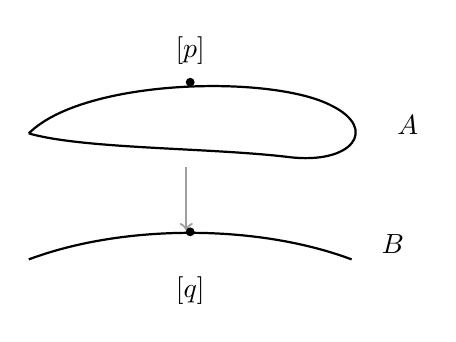
\begin{tikzpicture}[scale=1.0,line width=0.8pt]
  \draw (-2.0,1.25)
        .. controls (-1.3,1.95) and (1.1,2.0) .. (1.85,1.6)
        .. controls (2.45,1.3) and (2.1,0.85) .. (1.3,0.95)
        .. controls (0.3,1.07) and (-1.3,1.05) .. (-2.0,1.25);
  \fill (0.05,1.9) circle (1.6pt);
  \node at (0.05,2.3) {$[\mathfrak{p}]$};
  \node[anchor=west] at (2.55,1.35) {$\Spec A$};
  \draw[gray!75,->] (0,0.82) -- (0,0.02);
  \draw (-2.0,-0.35) .. controls (-0.8,0.1) and (0.9,0.1) .. (2.1,-0.35);
  \fill (0.05,0.0) circle (1.6pt);
  \node[anchor=west] at (2.35,-0.15) {$\Spec B$};
  \node at (0.05,-0.75) {$[\mathfrak{q}]$};
\end{tikzpicture}
\caption{Lying Over 定理~8.2.5 的一幅图：若 $\phi\colon B\to A$ 是\trIntegralExtension{}，则 $\Spec A\to\Spec B$ 是满的。（依原书手绘图重绘。）}\label{fig:lying-over-picture}
\end{figure}

下面这道练习为证明作好了准备。

\begin{exercise}[\hard]\label{ex:integral-field-case}
证明：$A$ 是\trField{}时的特例可以翻译为：若 $B\subset A$ 是\trSubring{}而 $A$ 在 $B$ 上\trIntegral，则 $B$ 是\trField。请证明它。（提示：你必须证明 $B$ 中一切非零元素都在 $B$ 中有\trInverseElement。这里是一个开头：若 $b\in B$，则 $1/b\in A$，而它满足某条在 $B$ 上的\trIntegrality{}方程。）
\end{exercise}

\emph{\hard\ Lying Over 定理~8.2.5 的证明。}\ 我们先作一个归约：对 $\mathfrak{q}$ 作\trLocalization{}（\trIntegrality{}由\cref{ex:integrality-localization-quotient}(b) 得以保持），便可假设 $(B,\mathfrak{q})$ 是一个\trLocalRing。然后任取 $A$ 的一个\emph{极大}理想 $\mathfrak{p}$。考虑如下的图。
\[
\begin{tikzcd}[row sep=3em, column sep=4.2em]
A \ar[r] & A/\mathfrak{p} & \text{域} \\
B \ar[u, hook] \ar[r] & B/(\mathfrak{p}\cap B) \ar[u, hook] &
\end{tikzcd}
\]
右边的竖直箭头由\cref{ex:integrality-localization-quotient}(c) 知是一个\trIntegralExtension{}。由\cref{ex:integral-field-case}，$B/(\mathfrak{p}\cap B)$ 也是\trField，于是 $\mathfrak{p}\cap B$ 是\trMaximalIdeal，从而它就是 $\mathfrak{q}$。\hfill$\square$

\begin{exercise}[重要练习（\textbf{Going-Up} 定理）]\label{ex:going-up-theorem}
\begin{enumerate}[label=(\alph*)]
\item 设 $\phi\colon B\to A$ 是一个\trIntegral{}的环\emph{映射}（不必是\trIntegralExtension{}）。证明：若 $\mathfrak{q}_1\subset\mathfrak{q}_2\subset\cdots\subset\mathfrak{q}_n$ 是 $B$ 的素理想的一条链，而 $\mathfrak{p}_1\subset\cdots\subset\mathfrak{p}_m$ 是 $A$ 的素理想的一条链，使得诸 $\mathfrak{p}_i$「位于」诸 $\mathfrak{q}_i$ 之上（且 $1\le m<n$），则第二条链可以扩充成 $\mathfrak{p}_1\subset\cdots\subset\mathfrak{p}_n$，使得这一情形依然成立。（提示：先化归到 $m=1$、$n=2$ 的情形；再化归到 $\mathfrak{q}_1=(0)$ 与 $\mathfrak{p}_1=(0)$ 的情形；然后使用 Lying Over 定理~8.2.5。）
\item 给这条定理画一幅图（与图~\ref{fig:lying-over-picture} 相仿）。
\end{enumerate}
\end{exercise}

也有与它们类似的「Going-Down」型结果（所需的假设颇为不同）；例如参看定理~12.2.12 与\mbox{练习~24.5.E}。

\textbf{8.2.7.\ \trNakayama{}引理。}

引理~8.2.1 证明中的那个巧招，还可以用来很快地证明\trNakayama{}引理——往后我们会一用再用。这个名字被用来称呼好几个互不相同却彼此相关的结果，我们在此一一讨论。（几何解读将在\mbox{练习~14.3.D}中给出。）趁这个巧招在我们脑中还热乎，不妨顺手把它证掉。

\textbf{8.2.8.\ \trNakayama{}引理版本~1。}\ ——\ \emph{设 $A$ 是一个环，$I$ 是 $A$ 的一个\trIdeal，$M$ 是一个有限生成的 $A$-\trModule，满足 $M=IM$。那么存在 $a\in A$，$a\equiv 1\pmod{I}$，使得 $aM=0$。（等价地：存在某个 $i\in I$，用 $i$ 作乘法在 $M$ 上诱导的是恒等映射：对一切 $m\in M$ 有 $im=m$。）}

\emph{证明。}\ 设 $M$ 由 $\mathsf{m}_1,\dots,\mathsf{m}_n$ 生成。那么由于 $M=IM$，存在诸 $a_{ij}\in I$ 使得 $\mathsf{m}_i=\sum_j a_{ij}\mathsf{m}_j$。于是
\begin{equation*}\tag{8.2.8.1}\label{eq:nakayama-adjugate-matrix}
(\mathrm{Id}_n-Z)
\begin{pmatrix}\mathsf{m}_1\\ \vdots\\ \mathsf{m}_n\end{pmatrix}
=0,
\end{equation*}
其中 $Z=(a_{ij})$。用 $\mathrm{adj}(\mathrm{Id}_n-Z)$ 左乘 \eqref{eq:nakayama-adjugate-matrix} 的两边，便得
\[
\det(\mathrm{Id}_n-Z)
\begin{pmatrix}\mathsf{m}_1\\ \vdots\\ \mathsf{m}_n\end{pmatrix}
=0.
\]
但当你把 $\det(\mathrm{Id}_n-Z)$ 展开时，由于 $Z$ 的元素都落在 $I$ 中，你得到的会是某个模 $I$ 同余于 $1$ 的东西。\hfill$\square$

说说你为什么要在意它。设 $I$ 含于 $A$ 的全部\trMaximalIdeal{}。（全体\trMaximalIdeal{}之交称为\textbf{\trJacobsonRadical{}}（Jacobson radical），但我们不会使用这个说法。作为对照，回想\trNilradical{}是 $A$ 的诸\emph{\trPrimeIdeal}之交。）%
此时，任何 $a\equiv 1\pmod{I}$ 都是可逆的。（此刻我们还没用上\trNakayama{}引理！）理由：否则 $(a)\neq A$，于是\trIdeal{} $(a)$ 含于某个\trMaximalIdeal{} $\mathfrak{m}$——但 $a\equiv 1\pmod{\mathfrak{m}}$，矛盾。既然 $a$ 可逆，我们便有下述结果。

\textbf{8.2.9.\ \trNakayama{}引理版本~2。}\ ——\ \emph{设 $A$ 是一个环，$I$ 是 $A$ 的一个含于全部\trMaximalIdeal{}的\trIdeal，$M$ 是一个有限生成的 $A$-\trModule。（最有趣的情形是 $A$ 为\trLocalRing{}而 $I$ 为其\trMaximalIdeal{}的情形。）设 $M=IM$。那么 $M=0$。}

\begin{exercise}[\trNakayama{}引理版本~3]\label{ex:nakayama-version-3}
设 $A$ 是一个环，$I$ 是 $A$ 的一个含于全部\trMaximalIdeal{}的\trIdeal。设 $M$ 是一个\emph{有限生成}的 $A$-\trModule，而 $N\subset M$ 是一个\trSubmodule。若 $N/IN\to M/IM$ 是\trSurjectiveMap，则 $M=N$。
\end{exercise}

\begin{exercise}[重要练习（\trNakayama{}引理版本~4：$M/\mathfrak{m}M$ 的生成元可提升为 $M$ 的生成元）]\label{ex:nakayama-version-4}
设 $(A,\mathfrak{m})$ 是一个\trLocalRing。设 $M$ 是一个有限生成的 $A$-\trModule，而 $f_1,\dots,f_n\in M$，使得（诸 $f_i$ 的像）生成 $M/\mathfrak{m}M$。那么 $f_1,\dots,f_n$ 生成 $M$。（特别地，取 $M=\mathfrak{m}$：只要有了 $\mathfrak{m}/\mathfrak{m}^2$ 的一组生成元，它们也就生成 $\mathfrak{m}$。）
\end{exercise}

\begin{exercise}[推广引理~8.2.1 的重要练习]\label{ex:integrality-faithful-module}
回想：若 $B$ 中在 $N$ 上以恒等映射作用的元素仅有 $1$（等价地，$B$ 中在 $N$ 上以零映射作用的元素仅有 $0$），就称 $B$-\trModule{} $N$ 是\textbf{\trFaithful{}的}（faithful）。设 $S$ 是环 $A$ 的一个\trSubring，$r\in A$。设存在一个\trFaithful{}的 $S[r]$-\trModule{} $M$，它作为 $S$-\trModule{}是有限生成的。证明：$r$ 在 $S$ 上\trIntegral。（提示：把\trNakayama{}引理版本~1（引理~8.2.8）的证明改动几个词。）
\end{exercise}

\begin{exercise}\label{ex:integral-closure-integrally-closed}
设 $A$ 是一个\trIntegralDomain，而 $\widetilde{A}$ 是 $A$ 在 $\mathrm{K}(A)$ 中的\textbf{\trIntegralClosure}，即 $\mathrm{K}(A)$ 中那些在 $A$ 上\trIntegral{}的元素——由\cref{ex:integral-elements-subalgebra}，它们构成一个\trSubalgebra{}。证明：$\widetilde{A}$ 在 $\mathrm{K}(\widetilde{A})=\mathrm{K}(A)$ 中是\trIntegrallyClosed{}的。
\end{exercise}


\section{态射上的一大堆有限性条件}

到本节结束之时，你将会见过以下几类\trMorphism：\trQuasicompact、\trQuasiSeparated、\trAffine、有限（finite）、\trIntegral、闭（closed）、（局部）有限型（(locally) of finite type）、\trQuasifinite{}（quasifinite）——或许还有（局部）有限表现（(locally) of finite presentation）。

\textbf{8.3.1.\ 拟紧与拟分离的\trMorphism。}

概形之间的\trMorphism{} $\pi\colon X\to Y$ 称为\textbf{\trQuasicompact}的，若对 $Y$ 的每个\trAffine\trOpenSubset{} $\mathsf{U}$，$\pi^{-1}(\mathsf{U})$ 都\trQuasicompact。（等价地，任何\trQuasicompact{}开子集的原像都\trQuasicompact。这也是几何学其他分支中正确的定义。）

我们将会喜欢这个观念，理由有二：(i) 有限集比起无限集自有好处（例如，整数的有限集必有最大元；再者，关于有限的对象可以归纳地证明）；(ii) 大多数合理的概形都将是\trQuasicompact{}的。

伴随着\trQuasicompactness{}而来的，是拟分离性这个古怪的观念。称\trMorphism{} $\pi\colon X\to Y$ 是\textbf{\trQuasiSeparated}的，若对 $Y$ 的每个\trAffine\trOpenSubset{} $\mathsf{U}$，$\pi^{-1}(\mathsf{U})$ 都是一个\trQuasiSeparated{}概形（\S5.1.1）。（等价地，任何\trQuasiSeparated{}开子集的原像都\trQuasiSeparated；我们不打算操心这件事的证明。这才是能推广到几何学其他分支的那种定义。）这条假设在定理中将会很有用，而且通常与\trQuasicompactness{}连用。（因此，「\trQuasicompact{}且\trQuasiSeparated」常被缩写作「qcqs」；参看 \S5.1.2。）几类有趣的\trMorphism（源为局部\trNoetherian、\trAffine、\trSeparated——分别参看\cref{ex:quasicompact-quasiseparated-source}(b)、练习~8.3.D 与\mbox{练习~11.2.D}）都是\trQuasiSeparated{}的，而有了「\trQuasiSeparated」一词，我们陈述定理时便能更加简练。\emph{重要注记：}我们将在 \S11.1.4（「拟分离＝拟紧对角」）中给出拟分离性的一个等价定义，它用起来会简单得多。

\textbf{8.3.A.（容易的练习）}\quad 证明：两个\trQuasicompact{}\trMorphism{}的\trComposition{}仍\trQuasicompact。（两个\trQuasiSeparated{}\trMorphism{}的\trComposition{}仍\trQuasiSeparated，这也成立——但不容易。你尽可以直接证明它，但无论如何，等我们对它有了更精巧的理解之后，它会轻易地随之而来；见 \S11.1.5。）

循着\trGrothendieck{}「重要的观念是\trMorphism{}的性质而非\trObject{}的性质」的哲学（\S8.0.1），我们可以把「\trQuasicompact 的（相应地，\trQuasiSeparated 的）概形」的定义重述为「在\trScheme{}的\trCategory{}中，它在\trFinalObject{} $\Spec\mathbb{Z}$ 之上\trQuasicompact（相应地，\trQuasiSeparated）的概形」（练习~7.3.J）。

\vkexsync{B}
\begin{exercise}[容易的练习]\label{ex:quasicompact-quasiseparated-source}
\begin{enumerate}[label=(\alph*)]
\item 证明：从\trNoetherian{}概形出发的任何\trMorphism{}都\trQuasicompact。
\item 证明：从\trQuasiSeparated{}概形出发的任何\trMorphism{}都\trQuasiSeparated。于是，由练习~5.3.A，从局部\trNoetherian{}概形出发的任何\trMorphism{}都\trQuasiSeparated。这样，只与局部\trNoetherian{}概形打交道的读者，尽可以把拟分离性当作一条\trStandingHypothesis{}（standing hypothesis）。
\end{enumerate}
\end{exercise}

\textbf{8.3.2.}\ \emph{\trhCaveat{}。}\quad \cref{ex:quasicompact-quasiseparated-source}的两部分或许会让你疑心：凡源与靶皆\trQuasicompact{}的\trMorphism{} $\pi\colon X\to Y$ 都必然\trQuasicompact。这是错的；你可以核验下面这个反例。设 $Z$ 是练习~5.1.K 中构造的那个非拟分离概形，并如练习~5.1.K 那样取 $X=\Spec k[x_1,x_2,\dots]$。那个显然的\trOpenEmbedding{} $\pi\colon X\to Z$（把 $X$ 认作粘出 $Z$ 的两块之一）不\trQuasicompact。（但等你见到\trCancellationTheorem{}~11.1.1 之后，立刻就会看出：从\trQuasicompact{}的源到一个\emph{\trQuasiSeparated}的靶的任何\trMorphism{}都必然\trQuasicompact。）

\vkexsync{C}
\begin{exercise}\label{ex:quasicompact-quasiseparated-affine-local}
（对两部分都显而易见的提示：\trAffineCommunicationLemma{}~5.3.2。）
\begin{enumerate}[label=(\alph*)]
\item （\trQuasicompactness{}是对目标仿射局部的。）证明：若存在由诸\trAffine\trOpenSet{} $\mathsf{U}_i$ 构成的 $Y$ 的一个\trCover{}，使得每个 $\pi^{-1}(\mathsf{U}_i)$ 都\trQuasicompact，则\trMorphism{} $\pi\colon X\to Y$ 是\trQuasicompact{}的。
\item （拟分离性是对目标仿射局部的。）证明：若存在由诸\trAffine\trOpenSet{} $\mathsf{U}_i$ 构成的 $Y$ 的一个\trCover{}，使得每个 $\pi^{-1}(\mathsf{U}_i)$ 都\trQuasiSeparated，则\trMorphism{} $\pi\colon X\to Y$ 是\trQuasiSeparated{}的。
\end{enumerate}
\end{exercise}

\textbf{8.3.3.\ \trAffine\trMorphism。}

称概形之间的\trMorphism{} $\pi\colon X\to Y$ 是\textbf{\trAffine}的，若对 $Y$ 的每个\trAffine\trOpenSet{} $\mathsf{U}$，$\pi^{-1}(\mathsf{U})$（解读为 $X$ 的一个\trOpenSubscheme）都是\trAffineScheme。平凡地，两个\trAffine{}\trMorphism{}的\trComposition{}仍\trAffine。

\textbf{8.3.D.（快速练习）}\quad 证明：\trAffine{}\trMorphism{}既\trQuasicompact{}又\trQuasiSeparated。（后者的提示：练习~5.1.G。）

\textbf{8.3.4.\ \trhProposition{}（一个\trMorphism{}的「仿射性」这一性质是对目标仿射局部的）。}\ ——\ \emph{设 $\pi\colon X\to Y$ 是一个\trMorphism。若存在 $Y$ 的一个由\trAffine\trOpenSet{} $\mathsf{U}$ 构成的\trCover{}，使得每个 $\pi^{-1}(\mathsf{U})$ 都\trAffine，则 $\pi$ 是\trAffine{}的。}

\emph{证明。}\ 我们把\trAffineCommunicationLemma{}~5.3.2 施于「$\pi$ 在其上是仿射的」这条条件。逐条核验我们的两条判据。第一，设 $\pi\colon X\to Y$ 在 $\Spec B$ 上仿射，即 $\pi^{-1}(\Spec B)=\Spec A$。则对任意 $s\in B$，$\pi^{-1}(\Spec B_s)=\Spec A_{\pi^\sharp s}$。（你可看出这是为什么吗？）

第二，设给了 $\pi\colon X\to\Spec B$ 与 $(s_1,\dots,s_n)=B$，诸 $X_{\pi^\sharp s_i}$ 都仿射（比如说为 $\Spec A_i$）。（回想定义~6.2.8：$X_{\pi^\sharp s_i}$ 是 $X$ 中 $\pi^\sharp s_i$ 不消失的开子集。）我们希望证明 $X$ 也是仿射的。令 $A=\Gamma(X,\OO_X)$。于是 $X\to\Spec B$ 可经由\trTautologicalMap{}（tautological map）$\alpha\colon X\to\Spec A$ 分解（它由那个（同构）映射 $A\to\Gamma(X,\OO_X)$ 产生，练习~7.3.G）。
\[
\begin{tikzcd}[row sep=3.2em, column sep=5.5em]
\bigcup_i X_{\pi^\sharp s_i}=X \ar[dr, "\pi"'] \ar[rr, "\alpha"] & & \Spec A \ar[dl, "\beta"] \\
& \bigcup_i D(s_i)=\Spec B &
\end{tikzcd}
\]
我们想证明 $\alpha$ 是一个\trIsomorphism。现在，$\beta^{-1}(D(s_i))=D(\beta^\sharp s_i)\cong\Spec A_{\beta^\sharp s_i}$（\trDistinguishedOpen{}的原像还是\trDistinguishedOpen），而 $\pi^{-1}(D(s_i))=\Spec A_i$。此外，由这些观念的仿射局部性（\cref{ex:quasicompact-quasiseparated-affine-local}），$X$ 既\trQuasicompact{}又\trQuasiSeparated，于是 Qcqs 引理~6.2.9 的诸假设得到满足。故由 Qcqs 引理~6.2.9，我们有诱导出的\trIsomorphism
\[
A_{\beta^\sharp s_i}=\Gamma(X,\OO_X)_{\beta^\sharp s_i}\cong\Gamma(X_{\beta^\sharp s_i},\OO_X)=A_i.
\]
于是 $\alpha$ 诱导\trIsomorphism{} $\Spec A_i\tilde{\longrightarrow}\Spec A_{\beta^\sharp s_i}$（环的\trIsomorphism{}诱导\trAffineScheme{}的\trIsomorphism，\cref{ex:scheme-isos-ring-isos}）。于是 $\alpha$ 在覆盖 $\Spec A$ 的所有 $\Spec A_{\beta^\sharp s_i}$ 上都是\trIsomorphism，从而 $\alpha$ 是\trIsomorphism。所以 $X\to\Spec A$ 是\trIsomorphism，即 $X$ 如愿地是\trAffine{}的。\hfill$\square$

\trAffine{}\trMorphism{}的仿射局部性（命题~8.3.4）有一些并不显然的推论，见下一道练习。

\textbf{8.3.E.（有用练习）}\quad 设 $Z$ 是\trAffineScheme{} $\Spec A$ 的一个由单个方程局部切出的\trClosedSubset。（换言之：$\Spec A$ 可以被一些更小的\trOpenSet{}覆盖，而在每个这样的\trOpenSet{}上，$Z$ 都由单个方程切出。）证明：$Z$ 的补集 $Y$ 是\trAffine{}的。（若 $Z$ 整体地由单个方程 $f$ 切出，哪怕只是在集合论的层面上，这件事也是清楚的；此时 $Y=\Spec A_f$。然而 $Z$ 并不总是这种形式；见 \S19.11.10。）

\textbf{8.3.5.\ 有限与\trIntegral{}的\trMorphism。}

在定义\trFinite{}与\trIntegral{}的\trMorphism{}之前，先给出一个值得放在心里的例子。若 $L/K$ 是一个\trFieldExtension，则 $\Spec L\to\Spec K$：(i) 总是\trAffine；(ii) 当 $L/K$ \trAlgebraic{}时是\trIntegral{}的；(iii) 当 $L/K$ 有限时是\trFinite{}的。

回想：若有\trRingMorphism{} $B\to A$ 使得 $A$ 是一个\trFinitelyGenerated{}的 $B$-\trModule，则我们称 $A$ 是一个\textbf{有限}（finite）$B$-\trAlgebra。这比「$A$ 是一个\trFinitelyGenerated{}的 $B$-\trAlgebra」要强。（「有限 $B$-代数」与「有限生成 $B$-代数」这两套术语如此相像，实在不幸。）称一个\trMorphism{} $\pi\colon X\to Y$ 是\textbf{有限}的，若对 $Y$ 的每个\trAffine\trOpenSet{} $\Spec B$，$\pi^{-1}(\Spec B)$ 都是一个有限 $B$-代数的谱。据定义，有限\trMorphism{}都是\trAffine{}的。

\textbf{8.3.F.（练习：\trFinite{}性这一性质是对目标仿射局部的）}\quad 证明：若存在由诸\trAffine\trOpenSet{} $\Spec A$ 构成的 $Y$ 的一个\trCover{}，使得每个 $\pi^{-1}(\Spec A)$ 都是某个\trFinite{} $A$-代数的谱，则\trMorphism{} $\pi\colon X\to Y$ 是\trFinite{}的。

下面四个例子会让你对有限\trMorphism{}找到一些感觉。在每个例子中，你都会注意到两件事。各种情形下，这些映射作为集合的映射总是\trFiniteToOne{}（finite-to-one）的；这一点我们将在练习~8.3.J 中一般地予以验证。
你还会注意到，这些\trMorphism{}作为\trTopologicalSpace{}的映射都是\textbf{闭}（closed）的，也就是说，\trClosedSet{}的像是\trClosedSet。
我们将在练习~8.3.L 中证明有限\trMorphism{}总是闭的（并在 \S9.3.5 中给出第二个证明）。直观上，你应当把「有限」想成「闭加上\trFiber{}有限」，尽管这并不全真。我们将在\mbox{定理~28.5.2}中把这话说精确。

\emph{例~1：\trBranchedCover{}（branched covers）。}\quad 考虑由 $u\mapsto p(t)$ 给出的\trMorphism{} $\Spec k[t]\to\Spec k[u]$，其中 $p(t)\in k[t]$ 是一个次数 $n$ 的多项式（见图~\ref{fig:branched-cover}）。
这是\trFinite{}的：$k[t]$ 作为 $k[u]$-\trModule{}由 $1$、$t$、$t^2$、……、$t^{n-1}$ 生成。

\begin{figure}[htbp]
\centering
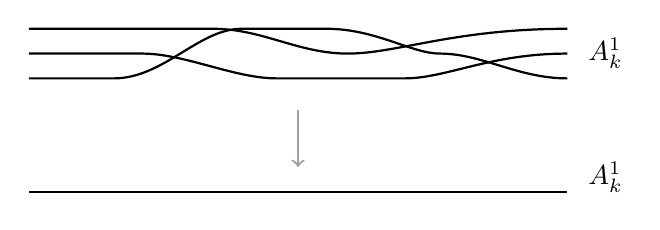
\begin{tikzpicture}[scale=0.9,line width=0.8pt]
  \draw (0,1.50) -- (2.6,1.50) .. controls (3.3,1.50) and (3.8,1.15) .. (4.5,1.15)
        .. controls (5.2,1.15) and (6.0,1.50) .. (7.6,1.50);
  \draw (0,1.15) -- (1.6,1.15) .. controls (2.2,1.15) and (2.9,0.80) .. (3.5,0.80)
        -- (5.3,0.80) .. controls (5.9,0.80) and (6.5,1.15) .. (7.6,1.15);
  \draw (0,0.80) -- (1.2,0.80) .. controls (1.9,0.80) and (2.4,1.50) .. (3.0,1.50)
        -- (4.2,1.50) .. controls (4.9,1.50) and (5.4,1.15) .. (5.8,1.15)
        .. controls (6.4,1.15) and (6.9,0.80) .. (7.6,0.80);
  \node[anchor=west] at (7.75,1.15) {$\mathbb{A}^1_k$};
  \draw[gray!75,->] (3.8,0.35) -- (3.8,-0.45);
  \draw (0,-0.80) -- (7.6,-0.80);
  \node[anchor=west] at (7.75,-0.60) {$\mathbb{A}^1_k$};
\end{tikzpicture}
\caption{由 $u\mapsto p(t)$ 给出的、以「$t$-线」盖住「$u$-线」的「\trBranchedCover{}」$\mathbb{A}^1_k\to\mathbb{A}^1_k$ 是\trFinite{}的。（依原书手绘图重绘，三股交叠为示意。）}\label{fig:branched-cover}
\end{figure}

\emph{例~2：闭嵌入（将很快于 \S9.1.1 中定义）。}\quad 设 $I$ 是\trRing{} $A$ 的一个\trIdeal，考虑由显然的映射 $A\to A/I$ 给出的\trMorphism{} $\Spec A/I\to\Spec A$（一个例子见图~\ref{fig:closed-embedding-spec-k}，取 $A=k[t]$，$I=(t)$）。这是一个\trFinite{}\trMorphism（$A/I$ 作为 $A$-\trModule{}由元素 $1\in A/I$ 生成）。

\begin{figure}[htbp]
\centering
\begin{tikzpicture}[scale=0.9,line width=0.8pt]
  \fill (0,1.70) circle (1.6pt);
  \draw[gray!75,->] (0,1.30) -- (0,0.35);
  \draw (-1.6,0) -- (1.6,0);
  \node at (0,-0.50) {$0$};
\end{tikzpicture}
\caption{由 $t\mapsto 0$ 给出的「闭嵌入」$\Spec k\to\Spec k[t]$ 是\trFinite{}的。（依原书手绘图重绘。）}\label{fig:closed-embedding-spec-k}
\end{figure}

\emph{例~3：正规化（将于 \S10.7 中定义）。}\quad 考虑\trMorphism{} $\Spec k[t]\to\Spec k[x,y]/(y^2-x^2-x^3)$，它对应于由 $x\mapsto t^2-1$、$y\mapsto t^3-t$ 给出的\trRingMorphism{} $k[x,y]/(y^2-x^2-x^3)\to k[t]$（请核验这是一个\trWellDefined{}的\trRingMorphism！）；见图~\ref{fig:normalization-nodal-cubic}。这是一个\trFinite{}\trMorphism，因为 $k[t]$ 作为 $\bigl(k[x,y]/(y^2-x^2-x^3)\bigr)$-\trModule{}由 $1$ 与 $t$ 生成。（图暗示：在靶的「\trNode{}」（node）之外，这是一个\trIsomorphism。
你可以核验这一点，办法是检验它在源中的 $D(t^2-1)$ 与靶中的 $D(x)$ 之间诱导了一个\trIsomorphism。我们还会一再地遇到这个例子！）

\begin{figure}[htbp]
\centering
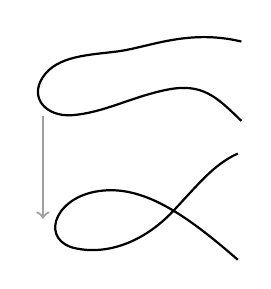
\begin{tikzpicture}[scale=0.9,line width=0.8pt]
  \draw (2.45,3.10) .. controls (1.70,3.28) and (1.15,3.02) .. (0.70,2.96)
        .. controls (0.30,2.91) and (-0.15,2.90) .. (-0.35,2.60)
        .. controls (-0.55,2.30) and (-0.30,2.04) .. (0.05,2.06)
        .. controls (0.50,2.09) and (0.90,2.32) .. (1.40,2.42)
        .. controls (1.90,2.52) and (2.10,2.32) .. (2.45,1.98);
  \draw[gray!75,->] (-0.35,2.05) -- (-0.35,0.60);
  \draw (2.40,0.02) .. controls (1.60,0.72) and (1.00,1.10) .. (0.38,0.98)
        .. controls (-0.22,0.86) and (-0.38,0.28) .. (0.12,0.18)
        .. controls (0.62,0.08) and (1.12,0.32) .. (1.48,0.70)
        .. controls (1.84,1.08) and (2.05,1.36) .. (2.40,1.52);
\end{tikzpicture}
\caption{\trNode{}三次曲线的「正规化」$\Spec k[t]\to\Spec k[x,y]/(y^2-x^2-x^3)$，由 $(x,y)\mapsto(t^2-1,\,t^3-t)$ 给出，是\trFinite{}的。（依原书手绘图重绘。）}\label{fig:normalization-nodal-cubic}
\end{figure}

\textbf{8.3.G.（重要练习：例~4，到 $\Spec k$ 的有限\trMorphism）}\quad 证明：若 $X\to\Spec k$ 是一个\trFinite{}\trMorphism，则 $X$ 是带\trDiscreteTopology{}的有限多个点的并，每个点的\trResidueField{}都是 $k$ 的一个\trFiniteFieldExtension；见图~\ref{fig:finite-morphism-spec-k}。（一个例子是 $\Spec\bigl(\mathbb{F}_8\times\mathbb{F}_4[x,y]/(x^2,y^4)\times\mathbb{F}_4[t]/(t^9)\times\mathbb{F}_2\bigr)\to\Spec\mathbb{F}_2$。）\emph{切莫}只引用某个花哨的定理了事！一条可能的进路：由\cref{ex:finite-algebra-domain-field}，任何是\trFinite{} $k$-代数的\trIntegralDomain{}必是\trField。设 $X=\Spec A$，证明 $A$ 的每个\trPrimeIdeal{} $\mathfrak{p}$ 都是\trMaximalIdeal。证明 $\Spec A$ 的诸\trIrreducibleComponent{}都是\trClosedPoint。证明 $\Spec A$ 是\trFinite{}的，进而是离散的。证明 $A$ 的诸\trResidueField{} $A/\mathfrak{m}$ 都是 $k$ 的\trFiniteFieldExtension。（向\trQuasifinite{}\trMorphism{}的推广见\mbox{练习~8.4.D}。）

\begin{figure}[htbp]
\centering
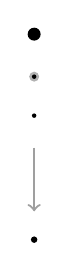
\begin{tikzpicture}[scale=0.9,line width=0.8pt]
  \fill (0,3.20) circle (2.6pt);
  \fill[gray!60] (0,2.60) circle (2.0pt);
  \fill (0,2.60) circle (0.9pt);
  \fill (0,2.05) circle (0.9pt);
  \draw[gray!75,->] (0,1.60) -- (0,0.70);
  \fill (0,0.30) circle (1.3pt);
\end{tikzpicture}
\caption{到 $\Spec k$ 的一个\trFinite{}\trMorphism{}的一幅图。更大的域被画成更大的点。（依原书手绘图重绘。）}\label{fig:finite-morphism-spec-k}
\end{figure}

\textbf{8.3.H.（容易的练习；参看\cref{ex:integrality-composition}）}\quad 证明：两个有限\trMorphism{}的\trComposition{}也有限。

\textbf{8.3.I.（练习：「到 $\Spec A$ 的有限\trMorphism{}是\trProjective{}的」）}\quad 设 $R$ 是一个 $A$-\trAlgebra。定义一个\trGradedRing{} $S_\bullet$ 如下：$S_0=A$，而对 $n>0$，$S_n=R$。（乘法结构是什么？提示：你知道如何把 $R$ 的元素彼此相乘，也知道如何把 $A$ 的元素与 $R$ 的元素相乘。）请描述一个\trIsomorphism{} $\Proj S_\bullet\tilde{\longrightarrow}\Spec R$。证明：若 $R$ 是一个\emph{有限} $A$-代数（即作为 $A$-\trModule{}\trFinitelyGenerated），则 $S_\bullet$ 是 $A$ 上\trFinitelyGenerated{}的\trGradedRing，从而 $\Spec R$ 是一个\trProjective{}的 $A$-\trScheme（\S4.5.10）。

于是有限\trMorphism{}既\trAffine（据定义）又\trProjective。逆命题也成立；见\mbox{推论~18.1.5}。

\textbf{8.3.J.（重要练习）}\quad 证明：有限\trMorphism{}有有限的\trFiber。（这是一道有用的练习，因为你终归得弄清楚怎样才能摸到一个\trMorphism{}的\trFiber{}里的点：给定 $\pi\colon X\to Y$ 与 $q\in Y$，$\pi^{-1}(q)$ 的点是什么？等我们在 \S10.3.2 中更细致地讨论过\trFiber{}之后，做起来会更容易——见注记~10.3.5——但现在就做会富于启发。）提示：设 $X=\Spec A$ 与 $Y=\Spec B$ 都是\trAffine{}的，而 $q=[\mathfrak{q}]$，那么对 $\mathfrak{q}$ 取商，便可把 $B$ 中位于 $\mathfrak{q}$ 之外的一切丢掉；证明原像是 $\Spec(A/\pi^\sharp\mathfrak{q}A)$。于是你便化归到了 $Y$ 是\trIntegralDomain{} $B$ 的谱、而 $[\mathfrak{q}]=[(0)]$ 为\trGenericPoint{}的情形。对 $(0)$ 作\trLocalization，便可把 $B$ 的其余诸点统统丢掉。证明原像是 $A$ 在 $\pi^\sharp(B\smallsetminus\{0\})$ 上\trLocalization{}后的谱。证明有限性这一条件在你所做的这些构造下得到保持，从而把问题化归到练习~8.3.G。

前两道练习表明：有限\trMorphism{}是\trProjective{}的，并且有有限的\trFiber。逆命题也成立；见\mbox{定理~18.1.6}。

关于有限性，\trFiber{}有限并非全部：值得放在心里的三个例子是例~8.3.6、练习~8.3.K 与图~19.1（图~\ref{fig:normalization-nodal-cubic} 的一个变体，它展示的\trMorphism{}是\trAffine{}的、闭的、在点上一对一的、甚至是\trMonomorphism，却不有限）。

\textbf{8.3.6.}\ \emph{\trhExample{}。}\quad \trOpenEmbedding{} $\mathbb{A}^2_k\setminus\{(0,0)\}\to\mathbb{A}^2_k$ 有有限的\trFiber，却不\trAffine（因为 $\mathbb{A}^2_k-\{(0,0)\}$ 不是\trAffine{}的，\S4.4.1），从而不有限。

\textbf{8.3.K.（容易的练习）}\quad 证明：\trOpenEmbedding{} $\mathbb{A}^1_{\mathbb{C}}\setminus\{0\}\to\mathbb{A}^1_{\mathbb{C}}$ 有有限的\trFiber{}且\trAffine，但不有限。

\textbf{8.3.7.}\ \emph{\trhDefinition{}。}\quad 称概形间的\trMorphism{} $\pi\colon X\to Y$ 是\textbf{\trIntegral}的，若 $\pi$ 是\trAffine{}的，且对每个 $\Spec B\subset Y$（\trAffine\trOpenSubset），记 $\pi^{-1}(\Spec B)=\Spec A$，其所诱导的映射 $B\to A$ 是\trIntegral{}的\trRingMorphism。据\cref{ex:integrality-affine-cover}与\cref{ex:integrality-localization-quotient}以及\trAffineCommunicationLemma{}~5.3.2，这是对目标\trAffineLocal{}的一条条件。由\cref{ex:integrality-composition}，它对\trComposition{}保持。\trIntegral{}\trMorphism{}之所以有用，主要在于：由推论~8.2.2，有限\trMorphism{}都是\trIntegral{}的。注意逆命题不成立（反例即 $\Spec\overline{\mathbb{Q}}\to\Spec\mathbb{Q}$，讨论见推论~8.2.2 的陈述之后）。

\textbf{8.3.L.（练习）}\quad 证明：\trIntegral{}\trMorphism{}是闭的，即\trClosedSubset{}的像是闭的。（从而有限\trMorphism{}是闭的。第二个证明将在 \S9.3.5 中给出。）提示：化归到仿射情形。设\trRingMorphism{} $\pi^\sharp\colon B\to A$ 诱导了\trIntegral{}\trMorphism{} $\pi\colon\Spec A\to\Spec B$；设 $I\subset A$ 切出 $\Spec A$ 的一个\trClosedSet，并令 $J=(\pi^\sharp)^{-1}(I)$；注意 $B/J\subset A/I$，然后施以 Lying Over 定理~8.2.5。

\textbf{8.3.M.（不重要练习）}\quad 设 $B\to A$ 是\trIntegral{}的。证明：对任何\trRingMorphism{} $B\to C$，所诱导的映射 $C\to A\otimes_B C$ 是\trIntegral{}的。（提示：我们希望证明 $\sum_{i=1}^n a_i\otimes c_i\in A\otimes_B C$ 在 $C$ 上\trIntegral。用「有限多个 $a_i$ 各自在 $B$ 上\trIntegral」这一事实，然后再用\cref{ex:integral-elements-subalgebra}。）等我们知道了什么是「\trBaseChange」之后，这将蕴含：一个\trMorphism{}的\trIntegrality{}这一性质对\trBaseChange{}保持，见\mbox{练习~10.4.D(e)}。

\textbf{8.3.8.}\ \emph{\trIntegral{}\trMorphism{}的诸\trFiber。}\quad 与有限\trMorphism{}不同（练习~8.3.J），\trIntegral{}\trMorphism{}的\trFiber{}未必有限。（你能想出一个例子吗？）不过，等我们在 \S10.3.2 中把\trFiber{}当作\trTopologicalSpace（甚至概形）讲出个道理之后，你就可以核验（\mbox{练习~12.1.E}）：诸\trFiber{}具有「没有任何一点落在其他任何一点的闭包之中」这一性质。

\textbf{8.3.9.\ （局部）\trFiniteType{}的\trMorphism。}

称\trMorphism{} $\pi\colon X\to Y$ 是\textbf{\trLocally\trFiniteType}（locally of finite type）的，若对 $Y$ 的每个\trAffine\trOpenSet{} $\Spec B$ 与 $\pi^{-1}(\Spec B)$ 的每个\trAffine\trOpenSubset{} $\Spec A$，所诱导的\trMorphism{} $B\to A$ 把 $A$ 表成一个\trFinitelyGenerated{}的 $B$-代数。据 $B$-概形之\trFiniteType{}性的仿射局部性（\trAffineLocal，命题~5.3.3(b)），这等价于：$\pi^{-1}(\Spec B)$ 可以被一些\trAffine\trOpenSubset{} $\Spec A_i$ 覆盖，使得每个 $A_i$ 都是\trFinitelyGenerated{}的 $B$-代数。

称\trMorphism{} $\pi$ 是\textbf{\trFiniteType}（of finite type）的，若它\trLocally\trFiniteType{}且\trQuasicompact。翻译过来：对 $Y$ 的每个\trAffine\trOpenSet{} $\Spec B$，$\pi^{-1}(\Spec B)$ 可以被\emph{有限多个}\trOpenSet{} $\Spec A_i$ 覆盖，使得所诱导的\trMorphism{} $B\to A_i$ 把 $A_i$ 表成一个\trFinitelyGenerated{}的 $B$-代数。

\textbf{8.3.10.}\ \emph{语言学上的好奇。}\quad 惯常的做法是这样来命名性质的：$P$＝局部 $P$＋\trQuasicompact。两个例外是「\trRingedSpace」（\S7.3）与「\trFinitelyPresented」（\S8.3.13）。

例：「\trStructureMorphism」 $\mathbb{P}^n_A\to\Spec A$ 是\trFiniteType{}的，因为 $\mathbb{P}^n_A$ 被形如 $\Spec A[x_1,\dots,x_n]$ 的 $n+1$ 个\trOpenSet{}所覆盖。

我们早先在 \S5.3.6 中给出的「$k$ 上\trFiniteType{}的概形」（或「\trFiniteType{} $k$-概形」）的定义，如今成了这个更一般观念的特例：「概形 $X$ 在 $k$ 上\trFiniteType」这句话的意思是，我们给定了一个\trFiniteType{}的\trMorphism{} $X\to\Spec k$（即「\trStructureMorphism」）。

下面是\trFiniteType{}\trMorphism{}享有的几条性质。

\textbf{8.3.N.（练习：「\trLocally\trFiniteType」与「\trFiniteType」都是对目标仿射局部的）}\quad 证明：若存在由诸\trAffine\trOpenSet{} $\Spec B_i$ 构成的 $Y$ 的一个\trCover{}，使得每个 $\pi^{-1}(\Spec B_i)$ 在 $B_i$ 上\trLocally\trFiniteType，则\trMorphism{} $\pi\colon X\to Y$ 是\trLocally\trFiniteType{}的。于是「\trLocally\trFiniteType」与「\trFiniteType」这两个概念都是对目标仿射局部的。

\vkexsync{O}
\begin{exercise}[有限＝\trIntegral{}＋\trFiniteType]\label{ex:finite-integral-finite-type}
\begin{enumerate}[label=(\alph*)]
\item （较易）证明：有限\trMorphism{}是\trFiniteType{}的。
\item 证明：一个\trMorphism{}是\trFinite{}的，当且仅当它既是\trIntegral{}的又是\trFiniteType{}的。
\end{enumerate}
\end{exercise}

\vkexsync{P}
\begin{exercise}[不难但重要的数道练习]\label{ex:finite-type-basic-properties}
\begin{enumerate}[label=(\alph*)]
\item 证明：每个\trOpenEmbedding{}都\trLocally\trFiniteType，从而每个\trQuasicompact{}的\trOpenEmbedding{}都是\trFiniteType{}的。证明：到局部\trNoetherian{}概形中的每个\trOpenEmbedding{}都是\trFiniteType{}的。
\item 证明：两个\trLocally\trFiniteType{}\trMorphism{}的\trComposition{}仍\trLocally\trFiniteType。（于是，既然两个\trQuasicompact{}\trMorphism{}的\trComposition{}是\trQuasicompact{}的——容易的练习~8.3.A——两个\trFiniteType{}\trMorphism{}的\trComposition{}便是\trFiniteType{}的。）
\item 设 $\pi\colon X\to Y$ \trLocally\trFiniteType，而 $Y$ 局部\trNoetherian。证明：$X$ 也局部\trNoetherian。若 $\pi\colon X\to Y$ 是一个\trFiniteType{}\trMorphism{}，而 $Y$ \trNoetherian，证明：$X$ \trNoetherian。
\end{enumerate}
\end{exercise}

\textbf{8.3.Q.（练习）}\quad 设 $X$ 是 $\mathbb{F}_p$ 上的一个\trScheme。解释如何（不用\trAxiomOfChoice）定义一个\trEndomorphism{}（endomorphism）$F\colon X\to X$，使得对每个\trAffine\trOpenSubset{} $\Spec A\subset X$，$F$ 都对应于由 $f\mapsto f^p$（对一切 $f\in A$）给出的映射 $A\to A$。（\trMorphism{} $F$ 称为\textbf{绝对\trFrobenius{}态射}（absolute Frobenius morphism）。）证明：若 $X$ 在 $\mathbb{F}_p$ 上\trLocally\trFiniteType，则 $F$ 是\trFinite{}的。

\textbf{8.3.11.}\ \emph{较不重要的定义。}\quad 称\trMorphism{} $\pi\colon X\to Y$ 是\textbf{\trQuasifinite{}}（quasifinite）的，若它\trFiniteType，且对一切 $q\in Y$，$\pi^{-1}(q)$ 都是有限集。这个定义的要点在「\trFiber{}有限」这部分；「\trFiniteType」这条假设将保证这个观念「对\trFiberProduct{}保持」，见\mbox{练习~10.4.F}。

把练习~8.3.J 与\cref{ex:finite-integral-finite-type}(a) 结合起来，便知有限\trMorphism{}都是\trQuasifinite{}的。也有\trQuasifinite{}却不有限的\trMorphism{}，例如 $\mathbb{A}^2_k\setminus\{(0,0)\}\to\mathbb{A}^2_k$（例~8.3.6）。不过我们很快就会看到：到 $\Spec k$ 的\trQuasifinite{}\trMorphism{}是\trFinite{}的（\mbox{练习~8.4.D}）。一个有有限\trFiber{}却不\trQuasifinite{}的关键例子是 $\Spec\mathbb{C}(t)\to\Spec\mathbb{C}$。另一个是 $\Spec\overline{\mathbb{Q}}\to\Spec\mathbb{Q}$。（由「$\Spec\overline{\mathbb{Q}}\to\Spec\mathbb{Q}$ 不是\trFiniteType{}的」这一事实引起的有趣行为，见警告~10.1.5。）

\textbf{8.3.12.}\ \emph{如何想象\trQuasifinite{}\trMorphism。}\quad 若 $\pi\colon X\to Y$ 是局部\trNoetherian{}概形之间的一个\trFinite{}\trMorphism，则对任意\trQuasicompact{}的\trOpenSubset{} $\mathsf{U}\subset X$，所诱导的\trMorphism{} $\pi|_{\mathsf{U}}\colon\mathsf{U}\to Y$ 是\trQuasifinite{}的。事实上，\emph{每一个}合理的\trQuasifinite{}\trMorphism{}都以这种方式出现。（这句听上去简单的陈述，实则是一个深刻而重要的结果——\trZariskiMainTheorem{}（Zariski's Main Theorem）的一种形式；见\mbox{练习~28.5.F}。）
于是，设想\trQuasifinite{}性的正确方式是：一个有限映射，再去掉某些点（的一条\trClosed\trLocus）。

\textbf{8.3.13.}\ \extrahard\ \textbf{（局部）\trFinitelyPresented{}的\trMorphism。}

下面这个「\trLocally\trFiniteType」的变体，在非诺特情形很有用。

\textbf{8.3.14.}\ \emph{\trhDefinition{}。}\quad 称一个\trRing{} $A$ 是\trFinitelyPresented{}的 $B$-代数（或 $B\to A$ 是\trFinitelyPresented{}的），如果「$A$ 在 $B$ 上有有限多个生成元与有限多个关系」：
\[
A\cong B[x_1,\dots,x_n]\big/\bigl(f_1(x_1,\dots,x_n),\dots,f_r(x_1,\dots,x_n)\bigr).
\]
若 $B$ \trNoetherian，则\trFinitelyPresented{}与\trFiniteType{}是一回事（「关系有限多条」是白送的，练习~3.6.S），所以正常人根本不会在意。

\textbf{8.3.R.（练习：有限表现蕴涵总是有限表现——代数版本）}\quad 设 $A$ 为 $B[x_1,\dots,x_n]$ 对\trIdeal{} $(f_1,\dots,f_r)$ 取商所得之环（诸 $f_i\in B[x_1,\dots,x_n]$）。又设 $Y_1,\dots,Y_m$ 作为 $B$-代数生成 $A$，于是有一个\trSurjectiveMap{} $\phi\colon B[y_1,\dots,y_m]\twoheadrightarrow A$（$y_j\mapsto Y_j$）。证明：\trIdeal{} $\ker(\phi)\subset B[y_1,\dots,y_m]$ 是\trFinitelyGenerated{}的。提示：循引理~6.4.6 的证明。

\textbf{8.3.15.\ \trhLemma{}（$A$ 在 $B$ 上的\trFinitelyPresented{}是在 $A$ 中\trAffineLocal{}的性质）。}\ ——\ \emph{$B$-代数之为\trFinitelyPresented{}这一条件，满足\trAffineCommunicationLemma{}~5.3.2 的假设。}

\emph{证明。}\ （i）\trAffineCommunicationLemma{}的第一条假设，正是下面这道练习的内容。

\textbf{8.3.S.（练习）}\quad 设 $A=B[x_1,\dots,x_n]/(f_1,\dots,f_r)$，而 $g\in A$。证明：$A_g$ 是一个\trFinitelyPresented{}的 $B$-代数。（提示：它多了一个生成元、多了一条关系。）

（ii）（这段论证是我们关于有限表现的讨论中最难的部分。）设 $A$ 是一个 $B$-代数，$g_1,\dots,g_m\in A$ 满足 $(g_1,\dots,g_m)=A$，且诸 $A_{g_i}$ 在 $B$ 上\trFinitelyPresented。我们希望证明 $A$ 在 $B$ 上\trFinitelyPresented。诸 $A_{g_i}$ 在 $B$ 上\trFinitelyGenerated，于是由命题~5.3.3(b)，$A$ 在 $B$ 上\trFinitelyGenerated，设有\trSurjectiveMap{} $\phi\colon B[x_1,\dots,x_n]\twoheadrightarrow A$。我们将证明 $I:=\ker(\phi)$ 是 $B[x_1,\dots,x_n]$ 的一个\trFinitelyGenerated{}的\trIdeal。

由于 $(g_1,\dots,g_m)=A$，我们可以选取诸 $h_j\in A$，使得 $1=h_1g_1+\cdots+h_mg_m$。把诸 $h_j$ 与诸 $g_j$ 分别提升为 $B[x_1,\dots,x_n]$ 中的 $H_j$ 与 $G_j$。令 $G_0=1-H_1G_1-\cdots-H_mG_m$，则 $G_0\in I$，且 $(G_0,G_1,\dots,G_m)=1$ 于 $B[x_1,\dots,x_n]$ 中。

\textbf{8.3.T.（练习）}\quad 证明：$I_{G_j}$ 是 $B[x_1,\dots,x_n]_{G_j}=B[x_1,\dots,x_n,y_j]/(y_jG_j-1)$ 上的一个\trFinitelyGenerated{}\trModule。（$j=0$ 的情形不同，但容易——$I_{G_0}=(1)$！）提示：引理~8.3.R。

于是，由练习~6.4.A（「模的有限生成是一条仿射局部条件」），$I$ 是一个\trFinitelyGenerated{}的 $B[x_1,\dots,x_n]$-\trModule，也就是说，$I$ 是 $B[x_1,\dots,x_n]$ 的一个\trFinitelyGenerated{}的\trIdeal，此即所愿。\hfill$\square$

\textbf{8.3.16.}\ \emph{\trhDefinition{}。}\quad 称一个 $B$-\trScheme{} $X\to\Spec B$ 在 $B$ 上\textbf{\trLocally\trFinitelyPresented}（locally finitely presented），若存在一个仿射\trCover{} $X=\bigcup\Spec A_i$，使得每个 $A_i$ 都在 $B$ 上\trFinitelyPresented。由引理~8.3.15，这等价于：对 $X$ 的\emph{一切}\trAffine\trOpenSubset{} $\Spec A$，$A$ 都在 $B$ 上\trFinitelyPresented。

\textbf{8.3.U.（练习：「\trLocally\trFinitelyPresented{}\trMorphism」这一概念对目标是\trAffineLocal{}的）}\quad 设 $\pi\colon X\to Y$ 是概形间的一个\trMorphism。证明：当 $\Spec B\subset Y$ 取遍 $Y$ 的诸\trAffine\trOpenSubset{}时，「$\pi\colon\pi^{-1}(\Spec B)\to\Spec B$ 在 $\Spec B$ 上\trLocally\trFinitelyPresented」这一条件满足\trAffineCommunicationLemma{}的假设。（这比引理~8.3.15 显著容易。）

\textbf{8.3.17.}\ \emph{\trhDefinition{}。}\quad 称\trMorphism{} $\pi\colon X\to Y$ 是\textbf{\trLocally\trFinitelyPresented}（locally finitely presented；或\textbf{局部有限表现的}，locally of finite presentation）的，若对 $Y$ 的每个\trAffine\trOpenSet{} $\Spec B$，$\pi^{-1}(\Spec B)\to\Spec B$ 在 $\Spec B$ 上\trLocally\trFinitelyPresented。由练习~8.3.U，只需在 $Y$ 的单独一个仿射覆盖上检验即可。（于是这涵盖了定义~8.3.16。）

\vkexsync{V}
\begin{exercise}\label{ex:locally-finitely-presented-covers}
设 $\pi\colon X\to Y$ 是概形间的一个\trMorphism。
\begin{enumerate}[label=(\alph*)]
\item 证明：若 $\pi$ \trLocally\trFinitelyPresented，则对 $Y$ 的\emph{任意}\trOpenSubscheme{} $\Spec B$ 与 $X$ 的\emph{任意}满足 $\pi(\Spec A)\subset\Spec B$ 的\trAffine\trOpenSubscheme{} $\Spec A$，$A$ 都是一个\trFinitelyPresented{}的 $B$-代数。
\item 设 $\bigcup\Spec A_i=X$ 是 $X$ 的一个仿射开覆盖，而诸 $\Spec B_i$ 是 $Y$ 的满足 $\pi(\Spec A_i)\subset\Spec B_i$ 的\trAffine\trOpenSubset。设每个 $A_i$ 都在 $B_i$ 上\trFinitelyPresented。证明：$\pi$ \trLocally\trFinitelyPresented。
\end{enumerate}
\end{exercise}

\textbf{8.3.W.（练习）}\quad 证明：\trOpenEmbedding{}都\trLocally\trFinitelyPresented。

\textbf{8.3.X.（练习）}\quad 证明：两个\trLocally\trFinitelyPresented{}\trMorphism{}的\trComposition{}仍\trLocally\trFinitelyPresented。

\textbf{8.3.18.}\ \extrahard\ \emph{\trhRemark{}。}\quad 称\trMorphism{} $\pi\colon X\to Y$ 是\trLocally\trFinitelyPresented{}的，当且仅当：对 $Y$-概形的每个\trProjectiveSystem{}（projective system）$\{S_\lambda\}_{\lambda\in I}$（其中每个 $S_\lambda$ 都是\trAffineScheme），自然映射
\[
\colim_{\lambda}\,\Hom_Y(S_\lambda,X)\longrightarrow\Hom_Y\bigl(\underset{\lambda}{\lim}\,S_\lambda,\,X\bigr)
\]
是双射（参看 [Gr-EGA, IV$_3$, 8.14.2]）。把\trLocally\trFinitelyPresented{}\trMorphism{}刻画为「保持极限」的这一特征可能有用。

\textbf{8.3.19.}\ \emph{\trhDefinition{}。}\quad 称一个\trMorphism{}是\textbf{\trFinitelyPresented}（finitely presented；或\textbf{有限表现的}，of finite presentation）的，若它\trLocally\trFinitelyPresented、\trQuasicompact{}且\trQuasiSeparated。特别地，\trFinitelyPresented{}\trMorphism{}这一概念是对目标仿射局部的。

这条定义违反了「擦去『局部』就等于加上『拟紧且』」这条原则（注记~8.3.10）。但它的动机是好的：\trFinitelyPresented{}意味着「在一切可能的方面都有限」（每个仿射开集对应的代数有有限多个生成元、有限多个关系；这样的仿射开集有有限多个，它们盖住了全空间；而它们的交也被有限多个仿射开集盖住）——对一个并不真的诺特的概形而言，这就是你所能指望的全部了。\mbox{练习~10.3.H} 把这一点讲精确，并解释这个观念在实践中常常如何出现。

若 $Y$ 局部\trNoetherian，则\trLocally\trFinitelyPresented{}与\trLocally\trFiniteType{}是一回事，且\trFinitelyPresented{}与\trFiniteType{}是一回事。所以，如果你是个诺特型的人，就无须为这个观念操心。\footnote{译注：此处戏拟「只与诺特情形打交道的人」，与上文 8.3.14 的「正常人」相映成趣。}


\section{态射的像：谢瓦莱定理与消元理论}

在本节中，我们要回答一个问题——早在听到「代数几何」这个词之前，你恐怕就琢磨过它了。如果你手头有一批带不定系数的多元多项式方程，你自然会问：系数满足什么条件，（公共）解才存在。鉴于问题本质是代数的，你有理由指望答案也纯属代数——它不该是「随机」的，也不该掺进指数函数、余弦之类古怪的函数。你应当期望答案由「代数条件」给出。事实确实如此，而且这件事可以卓有成效地改述为簇或概形之映射的像的问题；换了这副面孔，它便由谢瓦莱定理~8.4.2 给出解答（更精细的证明见\S8.4.8）。作为推论，我们还顺带得到\trNullstellensatz（\cref{thm:hilbert-nullstellensatz}）的一个立竿见影的证明（\S8.4.3）。

在某些情形，像还要更漂亮。例如，有限态射的像总是闭的（\mbox{练习~8.3.L}）。我们将证明一条经典结果——\trFundamentalTheoremOfEliminationTheory{}（Fundamental Theorem of Elimination Theory）~8.4.10，它本质上把这条事实推广（如\S9.3.5 所解释的）到从射影空间出发的映射。

沿另一个方向，我们将看到：在某些好的境况下（「平坦」再多一点点；见\mbox{练习~24.5.G}），态射是开的（开子集的像是开的）；一个例子（你可以试着直接证明）便是 $\mathbb{A}^1_B\to\Spec B$。

\textbf{8.4.1.\ \trChevalley{}定理。}

若 $\pi\colon X\to Y$ 是概形间的态射，则把 $\pi$ 的像当\emph{集合}看，其含义是清楚的：取 $Y$ 中那些身为 $X$ 中点之像的点即可。我们知道，像可以是开的（开嵌入），也见过像是闭的情形，以及更一般地，局部闭（locally closed）的情形。
但它还可以更怪：考虑由 $(x,y)\mapsto(x,xy)$ 给出的态射 $\mathbb{A}^2_k\to\mathbb{A}^2_k$。其像是全平面挖去 $y$-轴、再把原点放回来（图~\ref{fig:constructible-image-xy}）。我们为此现象下一个定义。\trNoetherian\trTopologicalSpace{}的一个子集称为\textbf{\trConstructible{}子集}（constructible subset），如果它属于由子集组成的、满足下列三条的最小族：(i) 每个开集都在族中；(ii) 族中成员的有限交仍在族中；(iii) 族中成员的补集也在族中。例如，$(x,y)\mapsto(x,xy)$ 的像是\trConstructible{}的。


\begin{figure}[htbp]
\centering
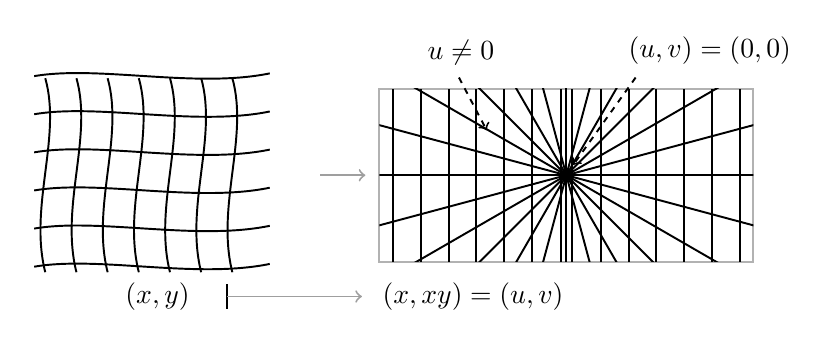
\begin{tikzpicture}[scale=0.88,line width=0.7pt]
  \begin{scope}[shift={(-5.9,1.25)}]
    \foreach \i in {0,...,6}
      \draw ({-1.62+0.45*\i},-1.4)
            .. controls ({-1.86+0.45*\i},-0.45) and ({-1.38+0.45*\i},0.55) ..
            ({-1.62+0.45*\i},1.4);
    \foreach \j in {0,...,5}
      \draw (-1.78,{-1.32+0.55*\j})
            .. controls (-0.85,{-1.16+0.55*\j}) and (0.55,{-1.5+0.55*\j}) ..
            (1.62,{-1.28+0.55*\j});
  \end{scope}
  \draw[gray!75,->] (-3.55,1.25) -- (-2.9,1.25);
  \draw[gray!60] (-2.7,0) rectangle (2.7,2.5);
  \begin{scope}
    \clip (-2.7,0) rectangle (2.7,2.5);
    \foreach \a in {0,15,...,345}
      \draw ({3.6*cos(\a)},{1.25+3.6*sin(\a)}) -- (0,1.25);
    \foreach \x in {-2.5,-2.1,...,-0.5} \draw (\x,0) -- (\x,2.5);
    \foreach \x in {0.5,0.9,...,2.5} \draw (\x,0) -- (\x,2.5);
    \draw (-0.08,0) -- (-0.08,2.5);
    \draw (0.08,0) -- (0.08,2.5);
  \end{scope}
  \fill (0,1.25) circle (1.7pt);
  \node[anchor=south west] at (-2.15,2.7) {$u\neq0$};
  \draw[dash pattern=on 2.2pt off 2.2pt,->] (-1.55,2.66) -- (-1.15,1.9);
  \node[anchor=south west] at (0.75,2.7) {$(u,v)=(0,0)$};
  \draw[dash pattern=on 2.2pt off 2.2pt,->] (1.0,2.66) -- (0.1,1.4);
  \node at (-5.9,-0.5) {$(x,y)$};
  \draw (-4.9,-0.32) -- (-4.9,-0.68);
  \draw[gray!75,->] (-4.9,-0.5) -- (-2.95,-0.5);
  \node[anchor=west] at (-2.8,-0.5) {$(x,xy)=(u,v)$};
\end{tikzpicture}
\caption{$(x,y)\mapsto(x,xy)=(u,v)$ 的像。（依原书手绘图重绘。）}\label{fig:constructible-image-xy}
\end{figure}

\begin{exercise}[练习：\trConstructible{}子集是\trLocally\trClosed{}子集的有限不交并]\label{ex:constructible-finite-disjoint-union}
回想：拓扑空间 $X$ 的一个子集称为\textbf{局部闭}（locally closed），如果它是一个开子集与一个闭子集的交。（等价地，它可以是闭子集的开子集，或者开子集的闭子集。日后要把这条推广到开子概形、闭子概形与\trLocally\trClosed{}子概形上去时，我们会遇到麻烦；见\mbox{练习~9.2.C}。）证明：诺特拓扑空间 $X$ 的一个子集是\trConstructible{}的，当且仅当它是\trLocally\trClosed{}子集的有限\trDisjointUnion。
\end{exercise}

作为推论，若 $X\to Y$ 是诺特拓扑空间之间的\trContinuousMap，则\trConstructible{}集的原像仍是\trConstructible{}集。（一条重要的评注：把「所论拓扑空间是诺特的」列为假设，唯一的原因是我们只在诺特的框架里定义了\trConstructible{}集。把可构造性（constructibility）这一概念推广到更一般的拓扑空间，见于\mbox{练习~10.3.I}。）

\begin{exercise}[容易的练习（用于\S8.4.3）]\label{ex:generic-point-not-constructible}
证明：$\mathbb{A}^1_k$ 的\trGenericPoint{}并不构成 $\mathbb{A}^1_k$ 的\trConstructible{}子集（其中 $k$ 是域）。
\end{exercise}

\begin{exercise}[练习（用于\mbox{练习~24.5.G}）]\label{ex:constructible-stable-specialization}
\begin{enumerate}[label=(\alph*)]
\item 证明：诺特概形的\trConstructible{}子集是闭的，当且仅当它在「\trSpecialization{}之下稳定」。更精确地：若 $Z$ 是诺特概形 $X$ 的\trConstructible{}子集，则 $Z$ 是闭的，当且仅当对每一对满足 $y_1\in\overline{y_2}$ 的点 $y_1$、$y_2$，只要 $y_2\in Z$，就有 $y_1\in Z$。「若」一方的提示：证明 $Z$ 能写成 $\coprod_{i=1}^{n}U_i\cap Z_i$，其中诸 $U_i\subset X$ 是开集，诸 $Z_i\subset X$ 是闭集。再证明：$Z$ 能写成 $\coprod_{i=1}^{n}U_i\cap Z_i$（其中的 $n$、$U_i$、$Z_i$ 尽可换作别的），使得每个 $Z_i$ 都\trIrreducible{}且与 $U_i$ 相交。然后用「\trSpecialization{}之下稳定」与诸 $Z_i$ 的\trGenericPoint{}证明：对一切 $i$ 都有 $Z_i\subset Z$，从而 $Z=\cup Z_i$。
\item 证明：诺特概形的\trConstructible{}子集是开的，当且仅当它在「\trGenerization{}之下稳定」。（提示：由 (a) 一行即得。）
\end{enumerate}
\end{exercise}

概形态射的像可以比\trConstructible{}集还要怪异。事实上，设 $S$ 是概形 $Y$ 的\emph{任意}子集，它都能充当某个态射的像：令 $X$ 为 $S$ 的全部点的剩余域之谱的\trDisjointUnion，令 $\pi\colon X\to Y$ 为自然映射。这相当病态；但在任何合理的情势下，像都不会比前例 $(x,y)\mapsto(x,xy)$ 中的像本质上更坏。谢瓦莱定理把这件事说得一清二楚。

\textbf{8.4.2.\ \trChevalley{}定理。}\ ——\ \emph{若 $\pi\colon X\to Y$ 是\trNoetherian\trScheme{}间的\trFiniteType\trMorphism，则任何\trConstructible{}集的像都可构造。特别地，$\pi$ 的像是\trConstructible{}的。}

（若你恰是会在意此事的少数派：向局部有限表现态射的推广，见\S10.3.8。）我们先给出几条或许出人意料的重要推论，再来讨论证明；出人意料之处在于，它们竟是一条看似十足几何、十足拓扑的定理的代数推论。第一条便是\trNullstellensatz{}的一个证明。

\textbf{8.4.3.}\ \emph{\trNullstellensatz（\cref{thm:hilbert-nullstellensatz}）的证明。}\quad 我们要证明：若 $K$ 是 $k$ 的\trFieldExtension{}且作为 $k$-\trAlgebra{}有限生成，比如说由 $x_1,\dots,x_n$ 生成，则它是域的\trFiniteFieldExtension。只需证明每个 $x_i$ 在 $k$ 上都是\trAlgebraic{}的。但若有某个 $x_i$ 在 $k$ 上不是\trAlgebraic{}的，我们便有一个环的包含映射 $k[x_i]\hookrightarrow K$，它对应于\trFiniteType{} $k$-\trScheme{}之间的一个\trDominant\trMorphism{} $\pi\colon\Spec K\to\mathbb{A}^1_k$。当然，$\Spec K$ 是单独一个点，故 $\pi$ 的像仅有一点。由谢瓦莱定理~8.4.2 与\cref{ex:generic-point-not-constructible}，$\pi$ 的像不是 $\mathbb{A}^1_k$ 的\trGenericPoint，于是 $\im(\pi)$ 是 $\mathbb{A}^1_k$ 的一个\trClosedPoint，从而 $\pi$ 不\trDominant。\hfill$\square$

同样的想法可用于下面的练习。

\begin{exercise}[练习（到域的\trQuasifinite{}态射皆有限）]\label{ex:quasifinite-to-field-finite}
设 $\pi\colon X\to\Spec k$ 是\trQuasifinite{}（quasifinite）态射。
证明：$\pi$ 是有限的。（提示：先处理仿射情形 $X=\Spec A$，其中 $A$ 在 $k$ 上有限生成。假设 $A$ 含有一个在 $k$ 上不\trAlgebraic{}的元素 $x$，也就是说，我们有一个包含映射 $k[x]\hookrightarrow A$。\mbox{练习~8.3.G} 或许可派上用场。）
\end{exercise}

\begin{exercise}\label{ex:finite-type-over-z-finite-residue}
设 $X$ 是 $\Spec\mathbb{Z}$ 上\trFiniteType{}的概形，而 $p$ 是 $X$ 的一个\trClosedPoint。证明：\trResidueField{} $\kappa(p)$ 是有限域。
\end{exercise}

\begin{exercise}[练习（对簇的映射，满性可在闭点上检验）]\label{ex:surjectivity-closed-points}
假设谢瓦莱定理~8.4.2。证明：仿射 $k$-簇之间的态射 $\pi\colon X\to Y$ 是满的，当且仅当它在闭点上是满的（即：$Y$ 的每个\trClosedPoint{}都是 $X$ 的某个\trClosedPoint{}的像）。（等到在定义~11.2.9 中一般地定义了簇之后，你会看到：你的论证无须改动便可照搬，只需抹去「仿射」这个形容词。）
\end{exercise}

\textbf{8.4.4.\ \trChevalley{}定理~8.4.2 的证明。}

\begin{exercise}\label{ex:chevalley-reduction}
\begin{enumerate}[label=(\alph*)]
\item 把谢瓦莱定理的证明化归到 $Y$ 为\trAffine{}的情形，比如说 $Y=\Spec B$。
\item 进一步化归到 $X$ 为\trAffine{}的情形，比如说 $X=\Spec B[t_1,\dots,t_n]/I$。
\item 进一步化归到 $X=\mathbb{A}^n_B=\Spec B[t_1,\dots,t_n]$ 的情形。
\item 进一步化归到 $X=\mathbb{A}^1_B=\Spec B[t]$ 的情形。
\end{enumerate}
\end{exercise}

至此，任务已化简为：给定 $\pi\colon X=\Spec B[t]\to\Spec B=Y$，证明 $X$ 的任何\trConstructible{}子集在 $Y$ 中的像可构造。由于\trConstructible{}集是\trLocally\trClosed{}子集的有限并（\cref{ex:constructible-finite-disjoint-union}——我们正处在诺特的情势中），只需证明：$X$ 的任何\emph{局部闭}子集 $Z$ 在 $Y$ 中的像可构造。

\textbf{8.4.5.}\ \emph{一个重要的特殊情形。}\quad 我们从 $Z$ 是 $X=\mathbb{A}^1_B$ 的\emph{闭}子集的情形入手，比如说
\[
Z=V(f_1(t),\dots,f_r(t))\text{，}\qquad\text{其中}\quad
f_i(t)=a_{id_i}t^{d_i}+\cdots+a_{i1}t+a_{i0}\text{，}
\]
诸 $a_{ij}\in B$，于是 $f_i(t)\in B[t]$，而 $d_i=\deg f_i(t)$。

现在 $Y=\Spec B$ 是诸\trLocally\trClosed{}子集 $Y_{\vec{e}}$ 的有限\trDisjointUnion，后者由 $\vec{e}=(e_1,\dots,e_r)$ 标号，其中 $e_i\in\mathbb{Z}$，$-1\le e_i\le d_i$；$Y_{\vec{e}}$ 是 $f_1(t),\dots,f_r(t)$ 分别具有「\trTrueDegree{}」（true degree）$e_1,\dots,e_r$ 的\trLocus：$f_i(t)$ 中 $t^{e_i}$ 的系数非零，而「更高次」的系数为零（在 $Y_{\vec{e}}$ 的各点处）。更精确地说：$Y_{\vec{e}}\subset Y$ 是使 $a_{ie_i}\neq0$、且对 $j>e_i$ 有 $a_{ij}=0$ 的\trLocus。（按此约定，零多项式的「\trTrueDegree{}」为 $-1$。）还要更精确的话，我们定义 $Y_{\vec{e}}:=\Spec B_{\vec{e}}$，其中
\[
B_{\vec{e}}:=\frac{B_{\prod_i a_{ie_i}}}{\left(a_{ij}\right)_{j>e_i}}\text{，}\qquad\text{于是}\quad
Y_{\vec{e}}=\Bigl(\mathop{\cap}\limits_{i}D(a_{ie_i})\Bigr)\cap
\Biggl(\mathop{\cap}\limits_{i,\ j>e_i}V(a_{ij})\Biggr)\text{。}
\]
若 $\vec{e}=(-1,\dots,-1)$，则
\begin{equation*}\tag{8.4.5.1}\label{eq:true-degree-fibration}
\pi^{-1}(Y_{\vec{e}})\xrightarrow{\ \pi\ }Y_{\vec{e}}
\end{equation*}
是满的（映射 \eqref{eq:true-degree-fibration} 即 $\Spec B_{(-1,\dots,-1)}[t]\to\Spec B_{(-1,\dots,-1)}$）；而若 $\vec{e}\neq(-1,\dots,-1)$，则 \eqref{eq:true-degree-fibration} 是一个有限态射，对应的环映射为
\[
B_{\vec{e}}\longrightarrow B_{\vec{e}}[t]\Bigm/\Bigl(t^{e_1}+\tfrac{a_{1(e_1-1)}}{a_{1e_1}}t^{e_1-1}
+\cdots+\tfrac{a_{10}}{a_{1e_1}},\ \dots,\ t^{e_r}+\tfrac{a_{r(e_r-1)}}{a_{re_r}}t^{e_r-1}
+\cdots+\tfrac{a_{r0}}{a_{re_r}}\Bigr)\text{。}
\]
（右边的环作为 $B_{\vec{e}}$-\trModule{}由 $1,t,\dots,t^{\max(e_i)}$ 生成。）由于有限态射的像是闭的（\mbox{练习~8.3.L}），$\pi(Z)\cap Y_{\vec{e}}$（即 \eqref{eq:true-degree-fibration} 的像）是 $Y$ 的\trLocally\trClosed{}子集，故当 $Z$ 为闭时，$\pi(Z)$ 确实可构造。我们的重要特殊情形至此完成。

\textbf{8.4.6.}\ 注意，使整条\trFiber{} $\pi^{-1}(q)$ 都含于 $Z$ 内的那些点 $q\in Y$ 所构成的\trLocus，即 $\{\,q\in Y\ :\ \pi^{-1}(q)\subset Z\,\}$，是 $Y$ 的一个\emph{闭}子集：它就是 $\Spec B_{(-1,\dots,-1)}=\Spec B/(a_{ij})$。我们把它记作 $\mathrm{FL}(Z)\subset Y$，称为「$Z$ 的\trFiber\trLocus」，但只在本次证明的余下部分中使用。\footnote{译注：FL 系 fibral locus（\trFibralLocus{}）的首字母缩写。}

\textbf{8.4.7.}\ 最后，若 $Z$ 是\emph{局部闭}的，则 $\overline{Z}\subset X$ 是闭的，故 $\pi(\overline{Z})$ 是 $Y=\Spec B$ 的\trConstructible{}子集。定义 $\delta Z:=\overline{Z}\smallsetminus Z$，这是 $X$ 的一个闭子集；由\S8.4.6，$\mathrm{FL}(\overline{Z})$ 与 $\mathrm{FL}(\delta Z)$ 都是 $Y$ 的闭子集。既然 $\mathrm{FL}(\overline{Z})\smallsetminus\mathrm{FL}(\delta Z)$ 含于 $\pi(Z)$，而 $\mathrm{FL}(\delta Z)$ 含于 $\pi(Z)$ 的\trComplement，只需对开子集 $Y':=Y\smallsetminus(\mathrm{FL}(\overline{Z})\cup\mathrm{FL}(\delta Z))\subset Y$ 证明结果即可。令 $\pi'\colon X'=\mathbb{A}^1_{Y'}\to Y'$ 为 $\pi$ 在 $Y'$ 上方的限制，令 $Z'=Z\cap\mathbb{A}^1_{Y'}$（它在 $Y'$ 上方\trQuasifinite{}），并令 $\delta Z'=\overline{Z'}\smallsetminus Z'\subset\mathbb{A}^1_{Y'}$（其中 $\overline{Z'}$ 是 $Z'$ 在 $\mathbb{A}^1_{Y'}$ 中的\trClosure）。

\begin{exercise}\label{ex:delta-z-generic-fibers}
证明：闭子集 $\delta Z'\subset\mathbb{A}^1_{Y'}$ 与 $\pi'$ 的任何一般纤维都不相交，也就是说，与 $Y'$ 的任何\trGenericPoint{}的\trInverseImage{}不相交。进而证明：$Y'$ 有一片\trDense{}的开子集，与\trConstructible{}集 $\pi'(\delta Z')$ 不相交。
\end{exercise}

至此，我们已在 $\Spec B$ 的一片\trDense{}开子集之上证明了结果。

\begin{exercise}\label{ex:chevalley-noetherian-induction}
借助诺特归纳，以某种足够严格的方式收尾谢瓦莱定理~8.4.2 的证明。
\end{exercise}

\hfill$\square$

\textbf{8.4.8.}\ \hard\ \textbf{\trEliminationOfQuantifiers{}}（elimination of quantifiers）。\quad 在数不清的语境中都会冒出来的一类基本问题是：一个方程组何时有解。设想，比方说，你手头有一些系数在代数闭域 $\bar{k}$ 上、关于变量 $x_1,\dots,x_n$ 的多项式，你把其中一部分置为零，另一部分置为非零。（早在你认识任何概形理论之前，这个问题就有着根本上的趣味！）那么，系数上存在一条代数条件，它会告诉你解是否存在。以显而易见的方式在 $\bar{k}^n$ 上定义\trZariskiTopology：闭子集由方程切出。（这条的一个温和推广出现在\mbox{练习~12.2.L}中。）

\begin{exercise}[练习（代数闭域上的\trEliminationOfQuantifiers{}）]\label{ex:elimination-quantifiers}
取定代数闭域 $\bar{k}$。设已给定
\[
f_1,\dots,f_p,\ g_1,\dots,g_q\in\bar{k}[W_1,\dots,W_m,X_1,\dots,X_n]\text{。}
\]
证明：存在 $\bar{k}^m$ 的一个（\trZariski-）\trConstructible{}子集 $Y$，使得
\begin{equation*}\tag{8.4.8.1}\label{eq:elimination-equalities}
f_1(w_1,\dots,w_m,X_1,\dots,X_n)=\cdots=f_p(w_1,\dots,w_m,X_1,\dots,X_n)=0
\end{equation*}
且
\begin{equation*}\tag{8.4.8.2}\label{eq:elimination-inequalities}
g_1(w_1,\dots,w_m,X_1,\dots,X_n)\neq0\qquad\cdots\qquad g_q(w_1,\dots,w_m,X_1,\dots,X_n)\neq0
\end{equation*}
有解 $(X_1,\dots,X_n)=(x_1,\dots,x_n)\in\bar{k}^n$，当且仅当 $(w_1,\dots,w_m)\in Y$。提示：若 $Z$ 是 $\bar{k}$ 上\trFiniteType{}的概形，其闭点记作 $Z^{\mathrm{cl}}$（「cl」既可以指 closed「闭」，也可以指 classical「经典」），则在拓扑空间的包含关系 $Z^{\mathrm{cl}}\subset Z$ 之下，$Z$ 上的\trZariskiTopology{}在 $Z^{\mathrm{cl}}$ 上诱导出\trZariskiTopology。注意：由\trNullstellensatz（\mbox{练习~5.3.F}），可以把 $(\mathbb{A}^p_{\bar{k}})^{\mathrm{cl}}$ 与 $\bar{k}^p$ 等同起来。若 $X$ 是 $\mathbb{A}^{m+n}$ 中由等式与不等式 \eqref{eq:elimination-equalities} 与 \eqref{eq:elimination-inequalities} 切出的\trLocally\trClosed{}子集，则我们有图
\begin{equation*}\tag{8.4.8.3}\label{eq:elimination-diagram}
\begin{tikzcd}[row sep=3em, column sep=3.4em]
X^{\mathrm{cl}} \ar[r, hook] \ar[d, "\pi^{\mathrm{cl}}"'] &
X \ar[r, hook, "loc.cl." description] \ar[d, "\pi"'] &
\mathbb{A}^{m+n} \ar[dl] \\
\bar{k}^{m} \ar[r, hook] & \mathbb{A}^{m}
\end{tikzcd}
\end{equation*}
其中 $Y=\im\pi^{\mathrm{cl}}$。由谢瓦莱定理~8.4.2，$\im\pi$ 可构造，从而 $(\im\pi)\cap\bar{k}^m$ 亦可构造。剩下要证的，是 $(\im\pi)\cap\bar{k}^m=Y$（即 $\im\pi^{\mathrm{cl}}$）。你不妨动用\trNullstellensatz。
\end{exercise}

它之所以名为「\trEliminationOfQuantifiers{}」，是因为它把「存在一个解」这个量词打发了。关于实数的相应陈述（其中还允许不等式），是\trTarski{}那条著名的\trRealClosedField{}（real closed field）\trEliminationOfQuantifiers{}定理的特例（例如参看 [Ta]）。

\textbf{8.4.9.\ \trFundamentalTheoremOfEliminationTheory{}。}

对射影空间（以及日后的射影态射）的情形，我们能比谢瓦莱做得更好（至少在描述\emph{闭}子集的像这件事上是如此）。

\textbf{8.4.10.\ \trhTheorem{}（\trFundamentalTheoremOfEliminationTheory{}）。}\ ——\ \emph{态射 $\pi\colon\mathbb{P}^n_A\to\Spec A$ 是\textbf{闭}的（\emph{把闭集送到闭集}）。}

注意，这里\emph{不需要}任何诺特假设。

大量的经典代数与几何作为特例包含在这条定理之中。这里给出几个例子。

首先，令 $A=k[a,b,c,\dots,i]$，考虑 $\mathbb{P}^2_A$（取坐标 $x$、$y$、$z$）中对应于 $ax+by+cz=0$、$dx+ey+fz=0$、$gx+hy+iz=0$ 的闭子集。我们要找的，是 $\Spec A$ 中这些方程具有非平凡解的\trLocus。这确实对应于一个\trZariski\trClosedSet——即
\[
\det\begin{pmatrix}a&b&c\\ d&e&f\\ g&h&i\end{pmatrix}=0
\]
之处。于是，行列式的观念便镶嵌在消元理论之中。

作为第二个例子，令 $A=k[a_0,a_1,\dots,a_m,b_0,b_1,\dots,b_n]$。考虑 $\mathbb{P}^1_A$（取坐标 $x$ 与 $y$）中对应于 $a_0x^m+a_1x^{m-1}y+\cdots+a_my^m=0$ 与 $b_0x^n+b_1x^{n-1}y+\cdots+b_ny^n=0$ 的闭子集。此时存在系数 $a_0,\dots,b_n$ 的一个多项式（即 $A$ 的一个元素），它在且仅在这两个多项式有公共非零根时才消失——这个多项式称为\emph{\trResultant{}}（resultant）。

更一般地，给定 $n+1$ 个变量的一批带不定系数的齐次方程，定理~8.4.10 蕴含：人们可以写下系数的一些方程，使它们恰好判定这些方程何时具有非平凡解。

\textbf{8.4.11.}\ \emph{\trFundamentalTheoremOfEliminationTheory{}~8.4.10 的证明。}\quad 设 $Z\hookrightarrow\mathbb{P}^n_A$ 是一个闭子集。我们要证明 $\pi(Z)$ 是闭的。

由 $\Proj A[x_0,\dots,x_n]$ 上\trZariskiTopology{}的定义（\S4.5.7），$Z$（在集合论意义上）由某些\trHomogeneous{}元素 $f_1,f_2,\dots\in A[x_0,\dots,x_n]$ 切出。我们要证明：$\Spec A$ 中位于 $\pi(Z)$ 内的那些点 $p$ 构成一个闭子集。等价地，我们要证明：使 $f_1,f_2,\dots$ 在 $\Proj\kappa(p)[x_0,\dots,x_n]$ 中具有公共零点的那些 $p$，构成 $\Spec A$ 的一个闭子集。

为给我们的论证提供动机，先考虑一个相关的问题。设 $S_\bullet:=k[x_0,\dots,x_n]$，而 $g_1,g_2,\dots\in k[x_0,\dots,x_n]$ 是\trHomogeneous{}多项式。我们如何判断 $g_1,g_2,\dots$ 在 $\Proj S_\bullet=\mathbb{P}^n_k$ 中有没有公共零点？

它们有公共零点，当且仅当在
\[
\mathbb{A}^{n+1}_k=\Spec S_\bullet
\]
中，它们（在集合论意义上）切出的东西多于原点，也就是说，在集合论意义上
\[
V(g_1,g_2,\dots)\not\subset V(x_0,\dots,x_n)\text{。}
\]
由闭子集与\trRadicalIdeal{}之间那个反转包含关系的双射（\cref{thm:closed-subsets-radical-ideals}），此话为真，当且仅当
\[
\sqrt{(g_1,g_2,\dots)}\not\supset\sqrt{(x_0,\dots,x_n)}\text{。}
\]
但 $(x_0,\dots,x_n)$ 是\trRadical，故此话为真，当且仅当
\[
\sqrt{(g_1,g_2,\dots)}\not\supset(x_0,\dots,x_n)\text{。}
\]
此话为真，当且仅当理想 $(x_0,\dots,x_n)$ 的生成元 $x_0,\dots,x_n$ 并非全部落在 $\sqrt{(g_1,g_2,\dots)}$ 中；而这又为真，当且仅当存在某个 $i$，使得 $x_i$ 的任何幂都不落在 $(g_1,g_2,\dots)$ 中。此话为真，当且仅当
\[
(x_0,\dots,x_n)^N\not\subset(g_1,g_2,\dots)\qquad\text{对一切 }N\text{。}
\]
（你看出这个蕴含为什么两个方向都成立吗？）这等价于
\[
S_N\not\subset(g_1,g_2,\dots)\qquad\text{对一切 }N\text{，}
\]
而这可以改写为
\begin{equation*}\tag{8.4.11.1}\label{eq:elimination-graded-map}
S_N\not\subset g_1S_{N-\deg g_1}\oplus g_2S_{N-\deg g_2}\oplus\cdots
\end{equation*}
对一切 $N$。换言之，这等价于下述陈述：$k$-线性映射
\[
S_{N-\deg g_1}\oplus S_{N-\deg g_2}\oplus\cdots\longrightarrow S_N
\]
不是满的。这个映射由一个有 $\dim S_N$ 行的矩阵给出。（它的列数可能是无限的，但这不会困扰我们。）要检验这个线性映射不满，只需检验所有「极大」的（$\dim S_N\times\dim S_N$）行列式都为零。（当然，这对一切 $N$ 都得检验。）于是，「$g_1,g_2,\dots$ 在 $\mathbb{P}^n_k$ 中没有公共零点」这一条件，就等同于检验（无可讳言的）无限多条方程。换言之，它是多项式 $g_1,g_2,\dots$ 的系数的一个\trZariski{}闭条件。

\begin{exercise}\label{ex:ftet-completion}
完成\trFundamentalTheoremOfEliminationTheory{}~8.4.10 的证明。（提示：循完全相同的论证，把 $k$ 换成 $A$，把诸 $g_i$ 换成诸 $f_i$。这为什么以及如何恰好证明了这条定理？若上一句话令你费解，不妨等到读到\S10.3.2，或者干脆现在就瞥一眼那里。）\hfill$\square$
\end{exercise}

注意，射影性在证明中至关重要：我们在本质处用到了\trGradedRing。还要注意，这个证明基本上不过是线性代数。

